\documentclass[xcolor=dvipsnames]{beamer}
%
% Choose how your presentation looks.
%
% For more themes, color themes and font themes, see:
% http://deic.uab.es/~iblanes/beamer_gallery/index_by_theme.html
%
\mode<presentation>
{
  \usetheme{default}      % or try Darmstadt, Madrid, Warsaw, ...
  \usecolortheme{default} % or try albatross, beaver, crane, ...
  \usefonttheme{default}  % or try serif, structurebold, ...
  \setbeamertemplate{navigation symbols}{}
  \setbeamertemplate{caption}[numbered]
} 

\usepackage[english]{babel}
\usepackage[utf8x]{inputenc}
\usepackage{animate}
\usepackage{dsfont}
\usepackage{minted}
\usepackage{tikz}
\usepackage{listings}
\usemintedstyle{default}

\definecolor{dark_blue}{RGB}{0,25,75}
\setbeamercolor{frametitle}{fg=White,bg=dark_blue!80}


\newcommand{\footlineB}{
\setbeamertemplate{footline}
{
  \leavevmode%
  \hbox{%
  \begin{beamercolorbox}[wd=.5\paperwidth,ht=7ex,dp=2ex,left]{title in head/foot}%
	\hspace{0.5cm} \vspace{-0.06cm} 
\includegraphics[width=.19\paperwidth]{images/edi-shield.pdf}
  \end{beamercolorbox}%
  \begin{beamercolorbox}[wd=.5\paperwidth,ht=7ex,dp=2ex,left,rightskip=.3cm]{title in head/foot}%
     \vspace{0.17cm}\hspace{-0.07cm}
     \textsf{\fontsize{4pt}{0cm}\selectfont
     \insertauthor  \newline 
	 \insertshortinstitute \hfill \insertframenumber
     }
    \end{beamercolorbox}%
    }%
  \vskip0pt%
}
}


\addtobeamertemplate{navigation symbols}{}{%
    \usebeamerfont{footline}%
    \usebeamercolor[fg]{footline}%
    \hspace{1em}%
    \insertframenumber/\inserttotalframenumber
}

\newcommand{\titlepageWhite}{ % % This block is for the white background title page
\setbeamertemplate{footline}
  {\hbox{%
    \begin{beamercolorbox}[wd=\paperwidth,dp=2ex,left]{title in head/foot}%
      %\hspace{-0.1cm} \vspace{0.52cm} 
      
      \vspace{-1.45cm}
      
\includegraphics[width=\paperwidth]{images/edi-shield.pdf}
    \end{beamercolorbox}%
      }%
    \vskip0pt%
  }
\defbeamertemplate*{title page}{customized}[1][]
  { \vspace{2cm}
  	\begin{beamercolorbox}[wd=0.9\paperwidth,dp=2ex,left]{author in head/foot}%
    %\usebeamerfont{title}{\LARGE\inserttitle\par}
    \usebeamerfont{title}\textcolor{dark_blue!90}{\LARGE\inserttitle}
    \par
    \bigskip
    \usebeamerfont{author}\textcolor{dark_blue!90}{\normalsize\insertauthor.}
    \par
    \smallskip
    \bigskip
    \usebeamerfont{date}\insertdate\par
    \end{beamercolorbox}
  }
}


\title[IISWC 2018 Presentation]{Characterising Across-Stack Optimisations for Convolutional Neural Networks}
\author{\textbf{J. Turner}, J. Cano, V. Radu, E. J. Crowley, M. O’Boyle, A. Storkey}
\institute{University of Edinburgh}
\date{}

\begin{document}

{\titlepageWhite
\begin{frame}
  \titlepage
\end{frame}
}

% Uncomment these lines for an automatically generated outline.
%\begin{frame}{Outline}
%  \tableofcontents
%\end{frame}


\section{Introduction}

\begin{frame}{Networks are large, and growing}

\begin{columns}

\column{0.5\textwidth}

\begin{figure}
    \centering
    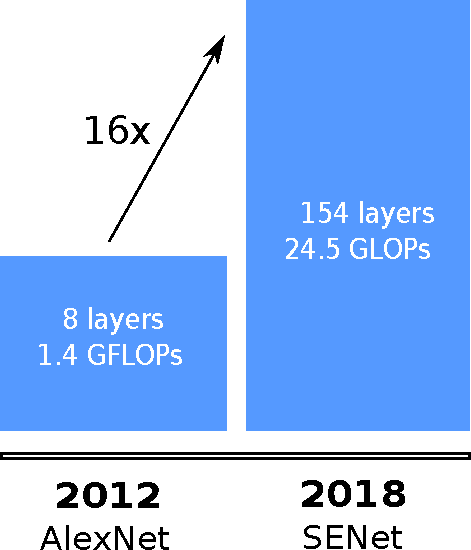
\includegraphics[width=5cm]{images/flop-growth.pdf}
    \label{fig:flop-growth}
    \caption{ImageNet winners}
\end{figure}

\column{0.5\textwidth}


\vspace{0.5cm}
\begin{itemize}
    \item High memory footprint
    \item Slow inference time 
    \item Large energy requirement
\end{itemize}

\end{columns}


\end{frame}


%\begin{frame}{Why Neural Networks?}

%\begin{figure}
%    \centering
%    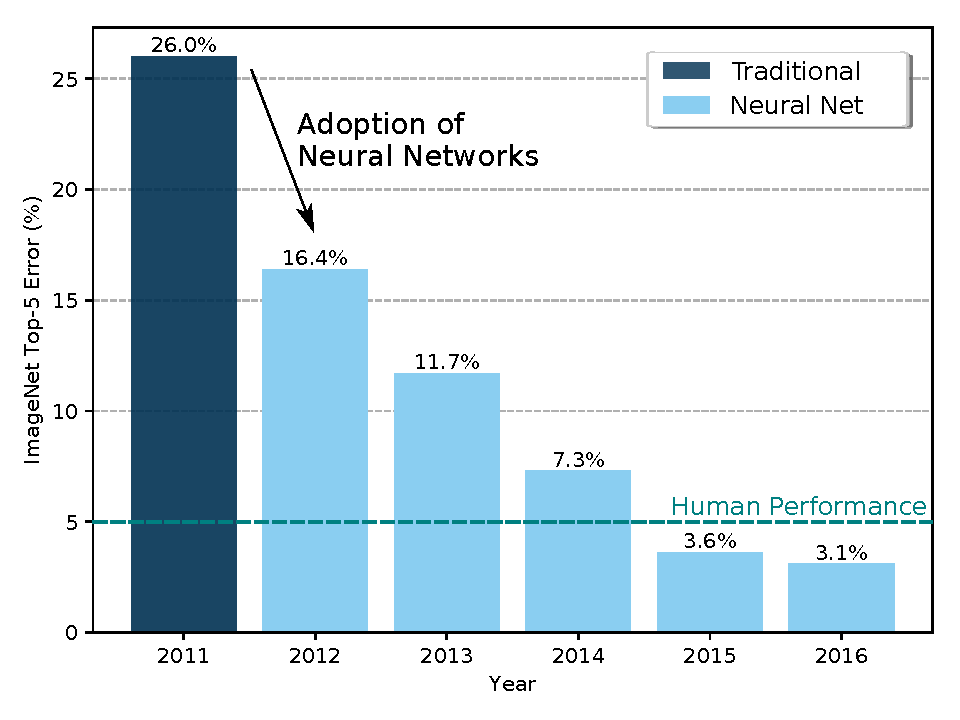
\includegraphics[width=\linewidth]{images/imagenet_results.pdf}
%\end{figure}


%\end{frame}


\section{Challenges for Deployment}

\subsection{Large Models}


\begin{frame}{Speedup does not align with expectations}

\begin{itemize}
	\item In state-of-the-art networks, up to \textbf{90\%} of weights are redundant
\end{itemize}

\begin{figure}
    \centering
    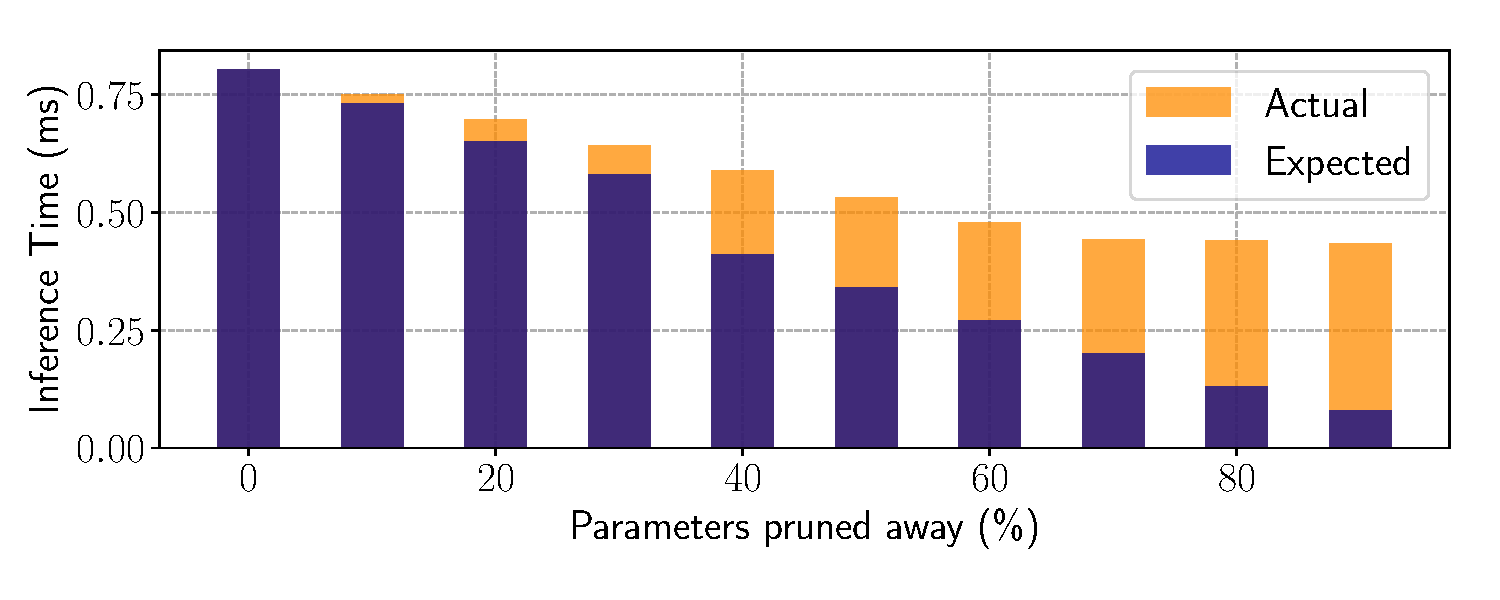
\includegraphics[width=10cm]{images/speedup.pdf}
\end{figure}



\end{frame}


\begin{frame}{Different hardware demands different compression}

\begin{figure}
    \centering
    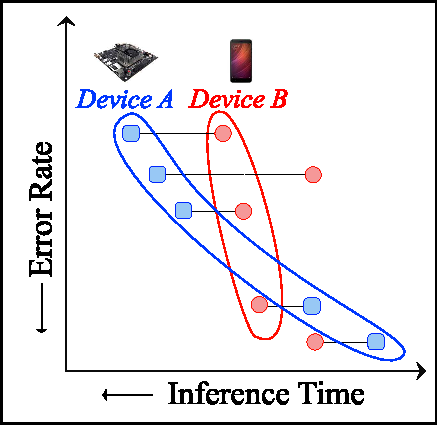
\includegraphics[width=0.6\linewidth]{images/pareto_efficiency.pdf}
\end{figure}

[Dong et. al, 2018. DPP-Net: Device-aware Progressive Search for Pareto-optimal Neural Architectures]
\end{frame}


\begin{frame}{The Deep Learning Inference Stack}
\begin{figure}
    \centering
    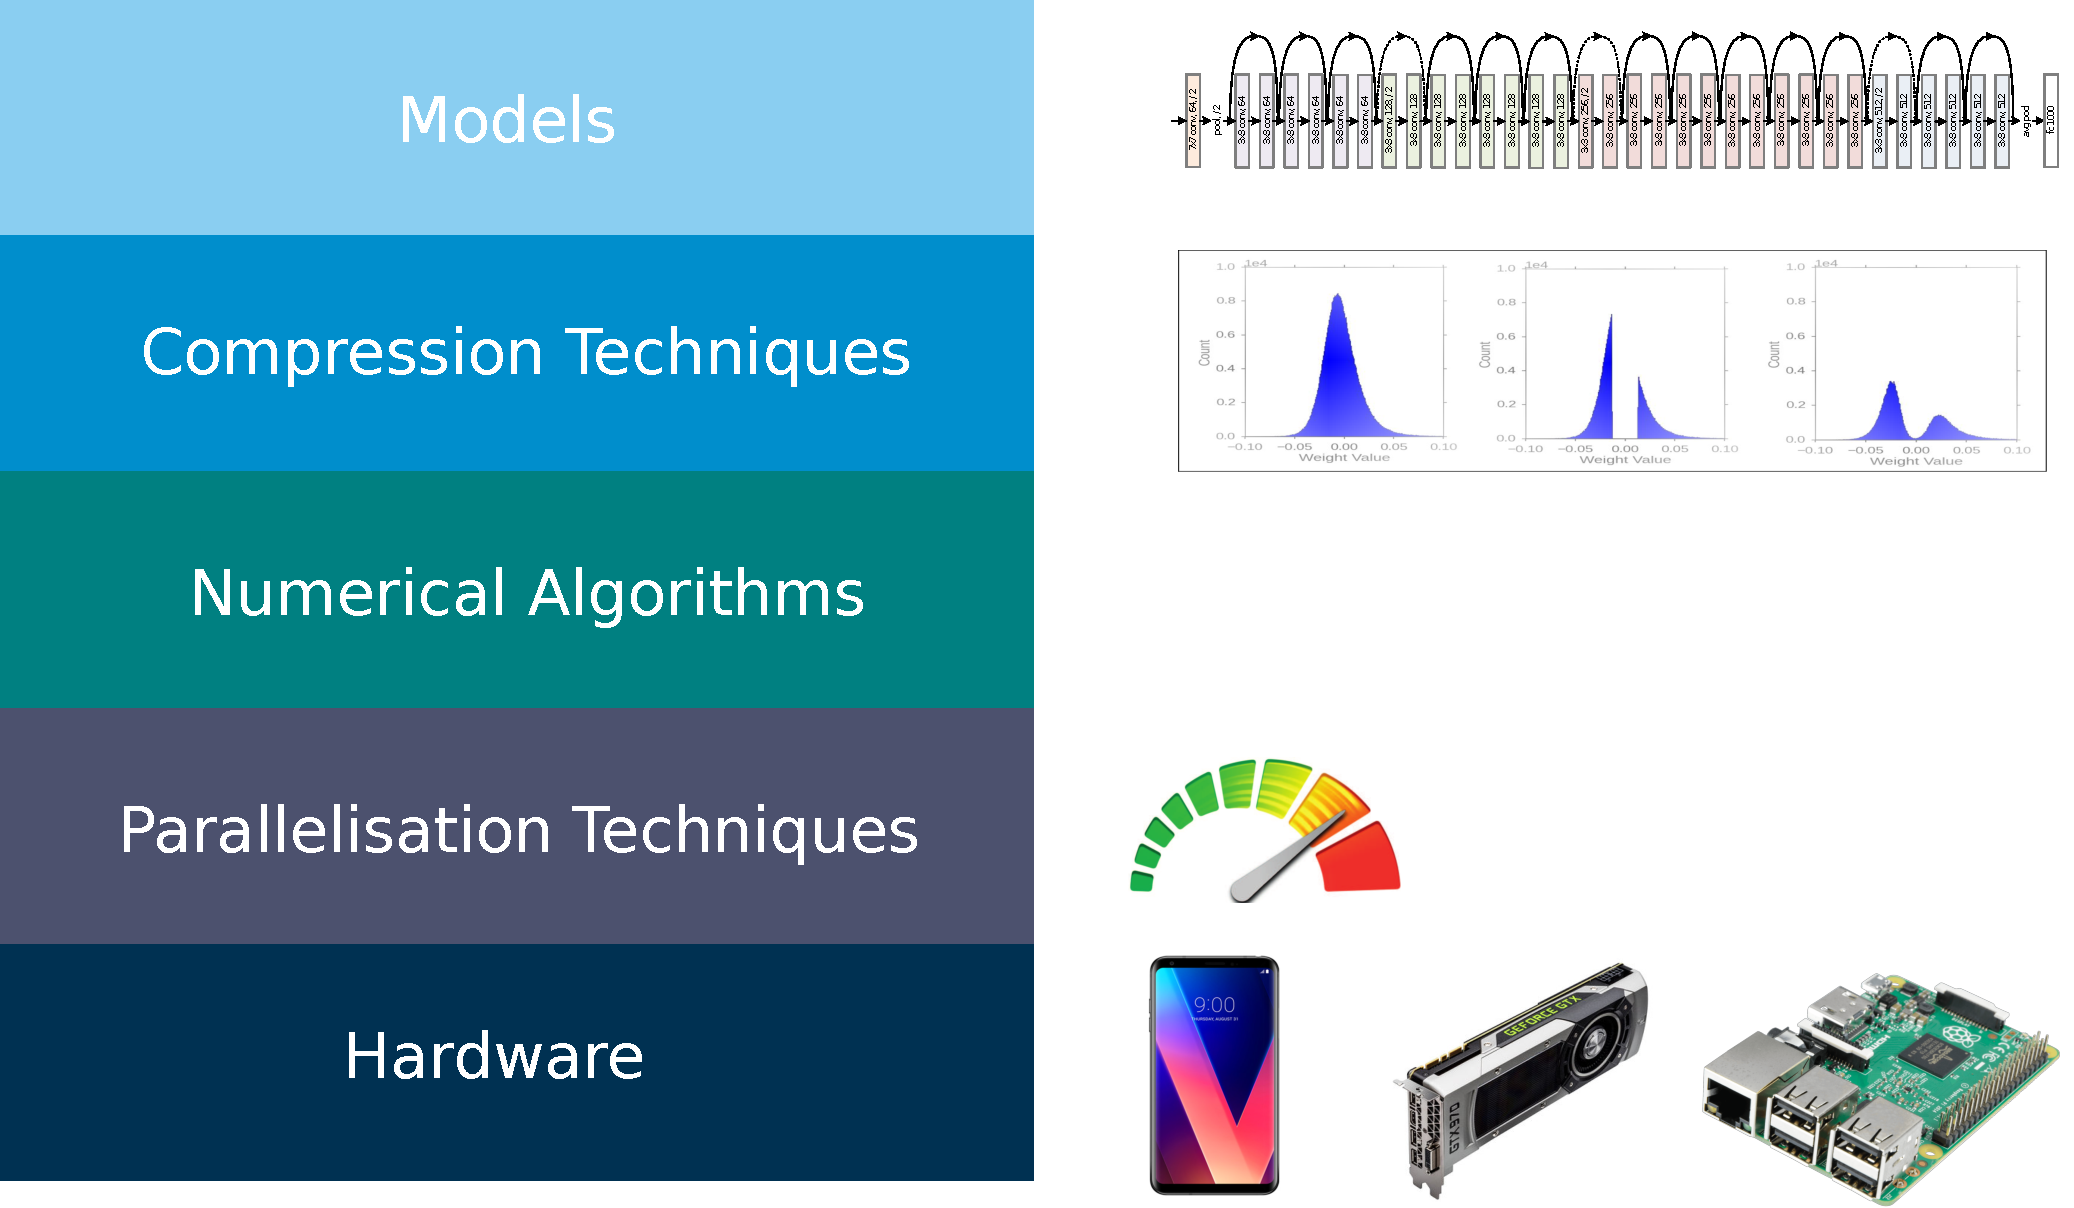
\includegraphics[width=\linewidth]{images/inference-stack.pdf}
\end{figure}
\end{frame}



\section{Background}

{
\setbeamercolor{background canvas}{bg=dark_blue!80}
\begin{frame}
    \centering
    \textcolor{white}{\LARGE Background}
\end{frame}
}


%\begin{frame}{Background: Neurons}

%\begin{figure}
%    \centering
%    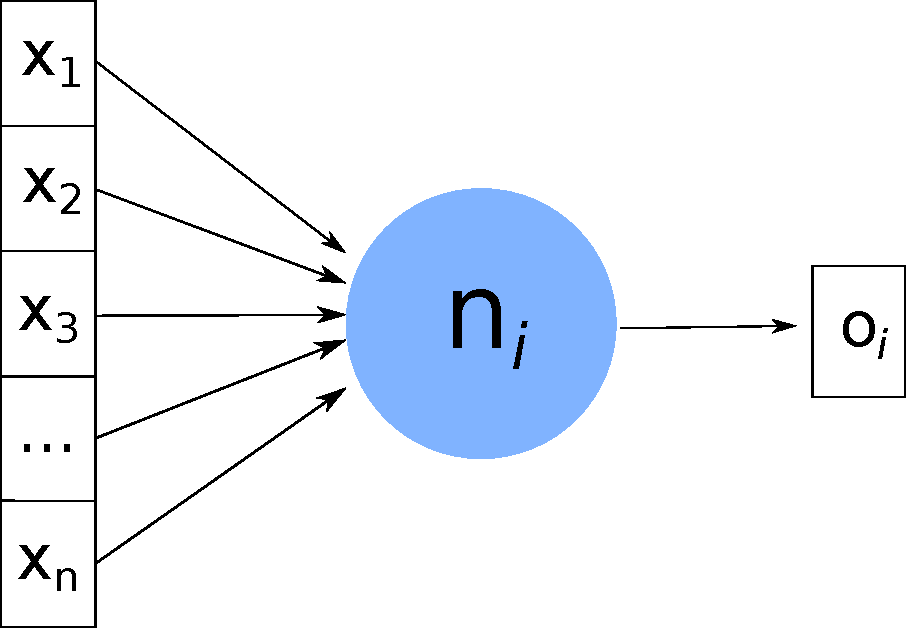
\includegraphics[width=0.8\textwidth]{images/neuron.pdf}
%\end{figure}

%\end{frame}


%\begin{frame}{Background: Affine Transform Neurons}

%Multiply each input element $x$ by a weight $w$ and add a scalar bias term $b$:

%\begin{figure}
%    \centering
%    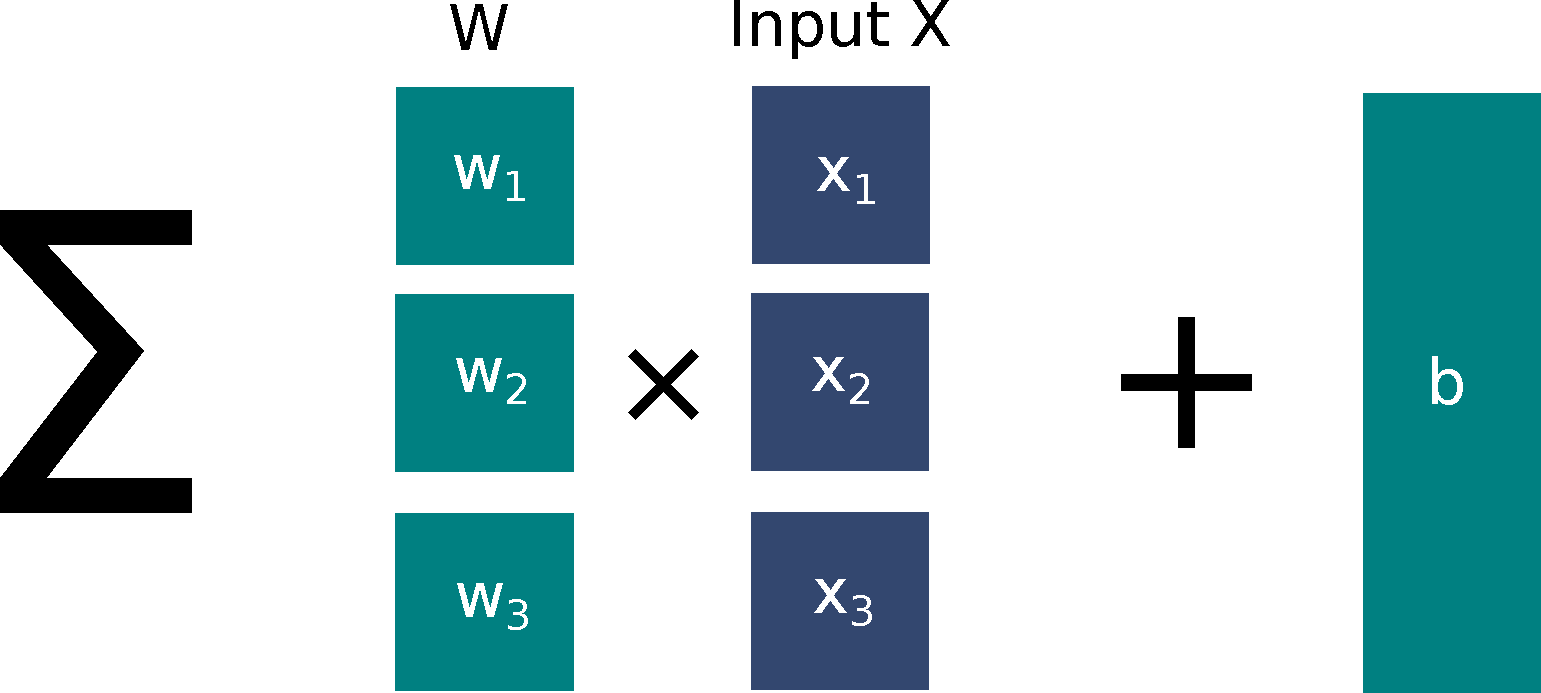
\includegraphics[width=0.8\linewidth]{images/affine_transform.pdf}
%\end{figure}

%\end{frame}

%\begin{frame}{Background: Layers}

%\begin{figure}
%    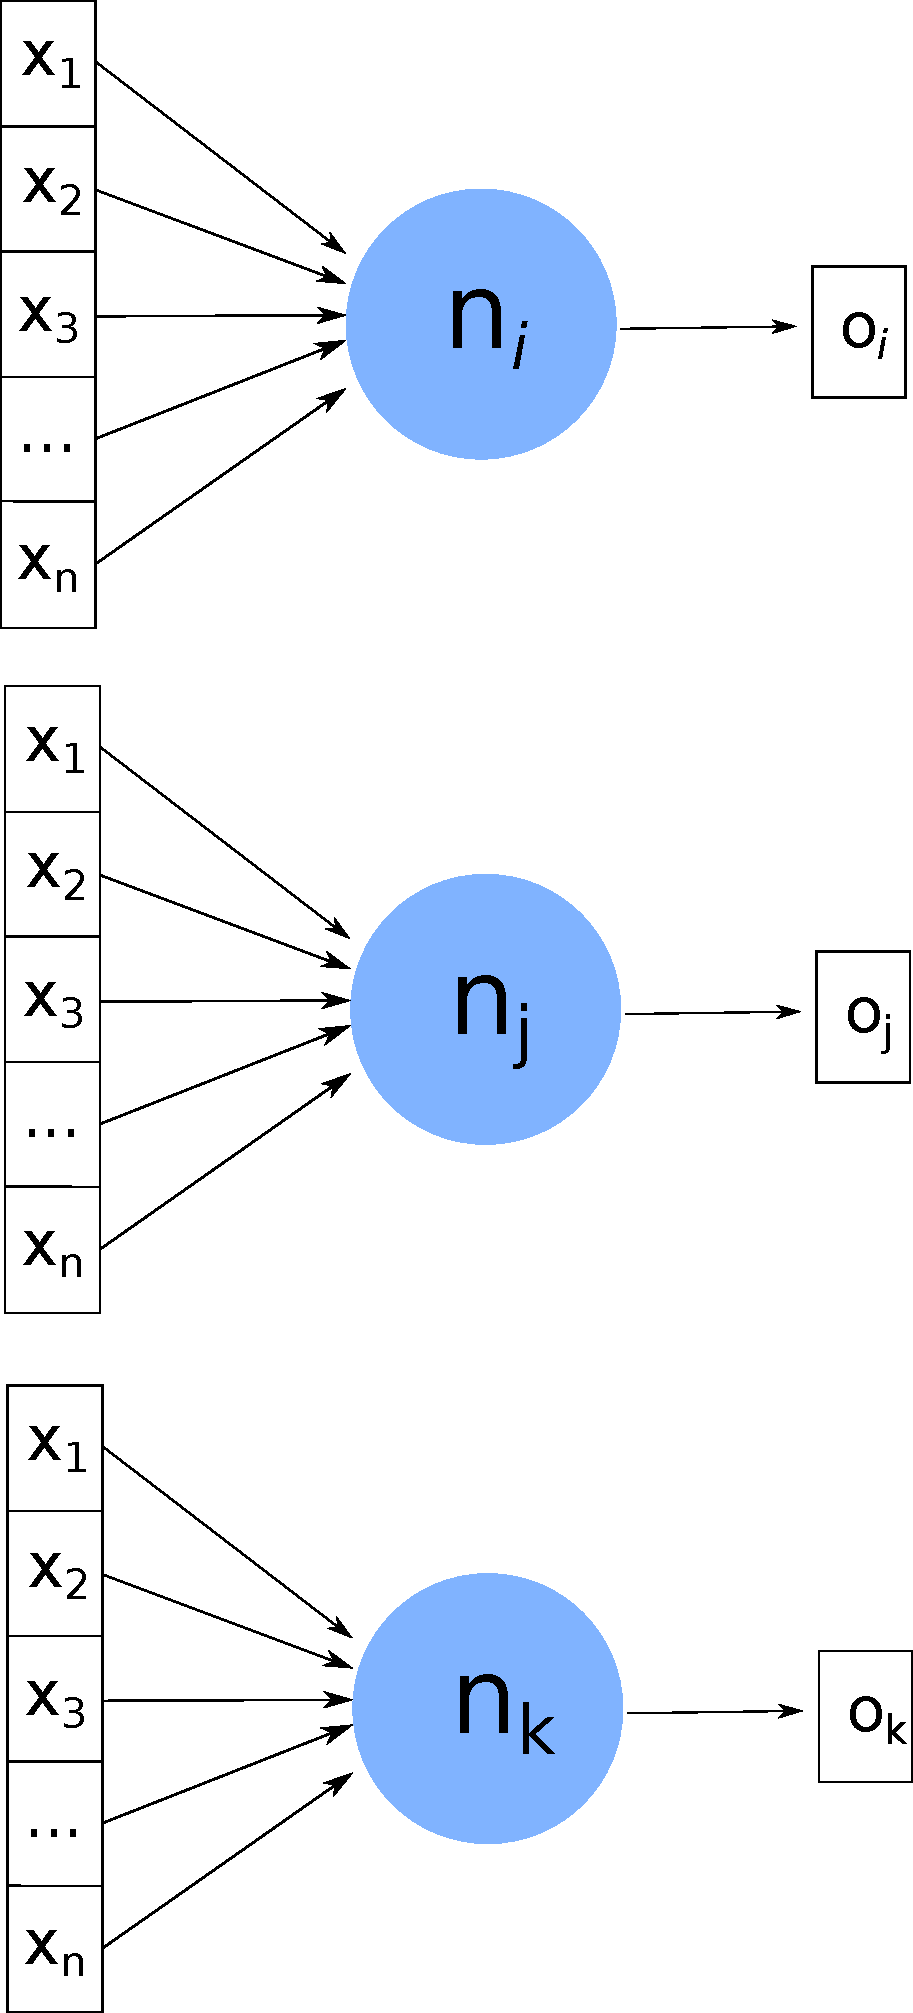
\includegraphics[width=3cm]{images/layer.pdf}
%\end{figure}

%\end{frame}


%\begin{frame}{Background: Neural Networks}

%\begin{figure}
%    \centering
%    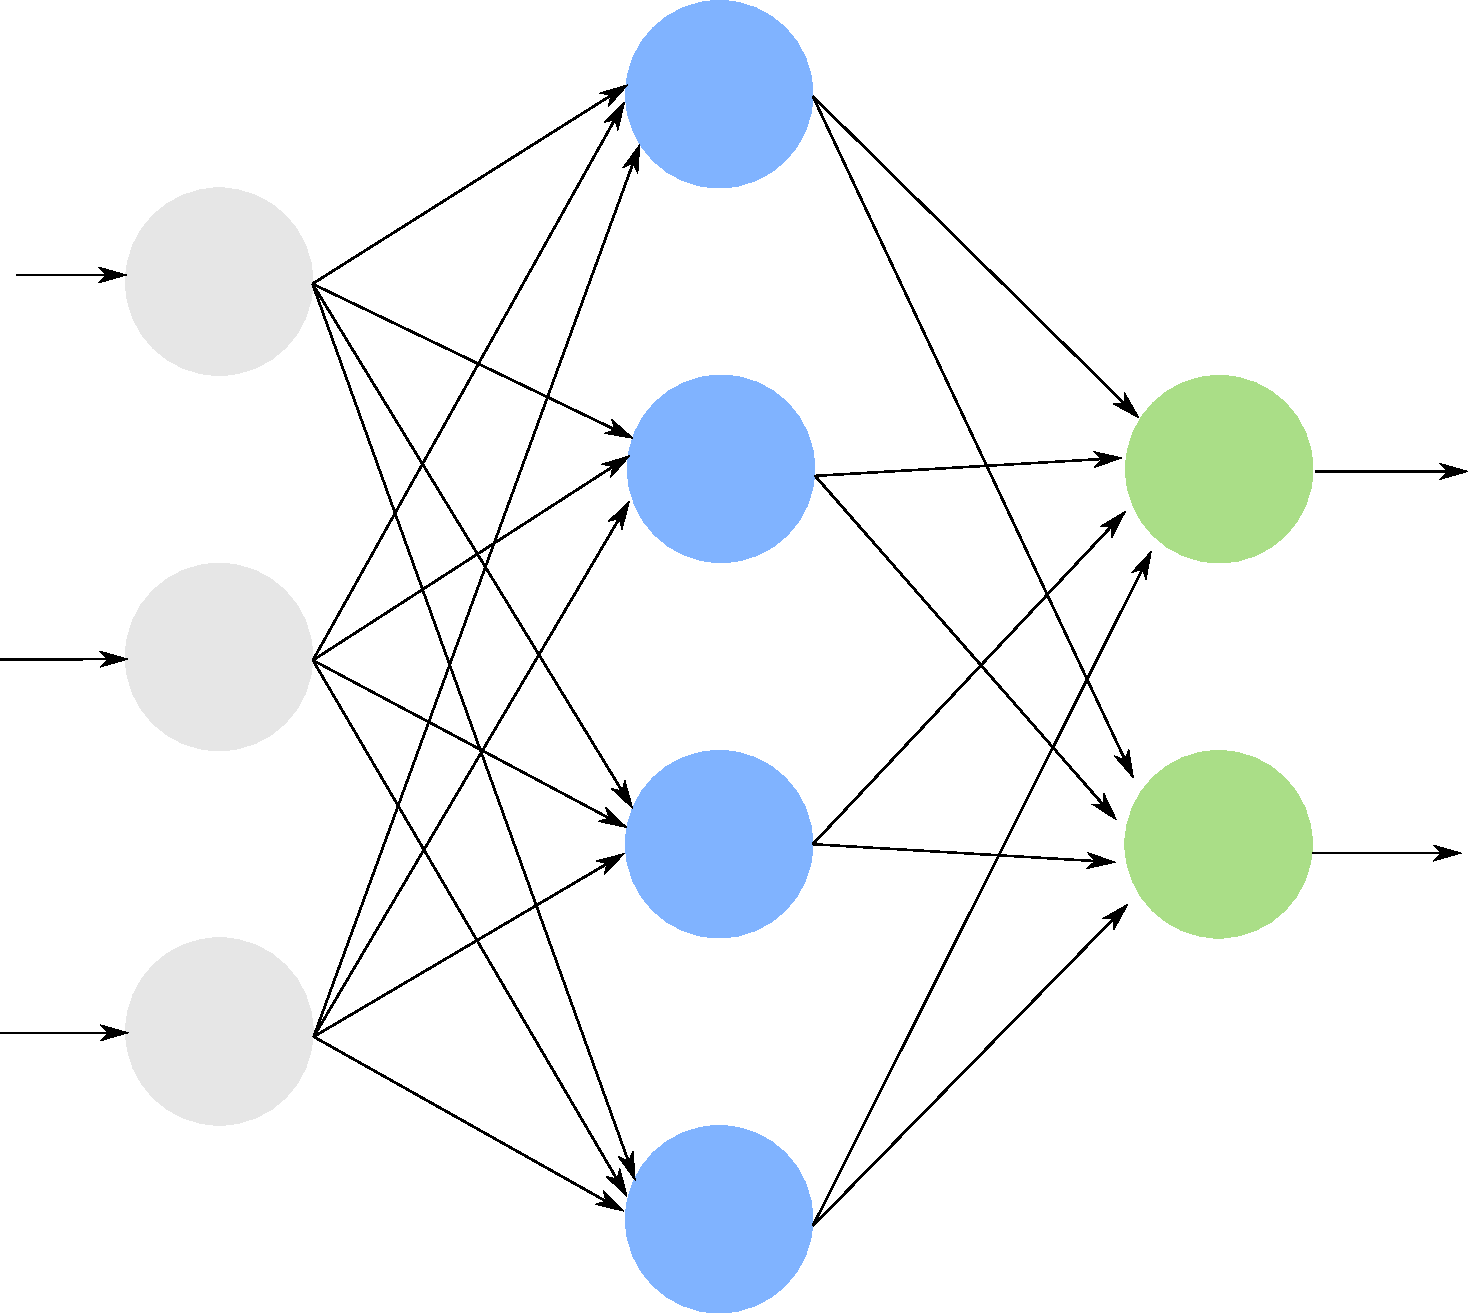
\includegraphics[width=0.6\linewidth]{images/neural_network.pdf}
%\end{figure}
%\end{frame}


%\begin{frame}{Background: Convolution Neurons}
%\centering
%\animategraphics[loop,controls,width=0.6\linewidth]{1}{images/arbitrary_padding_no_strides_0}{0}{3}

%\begin{figure}
%    \centering
%    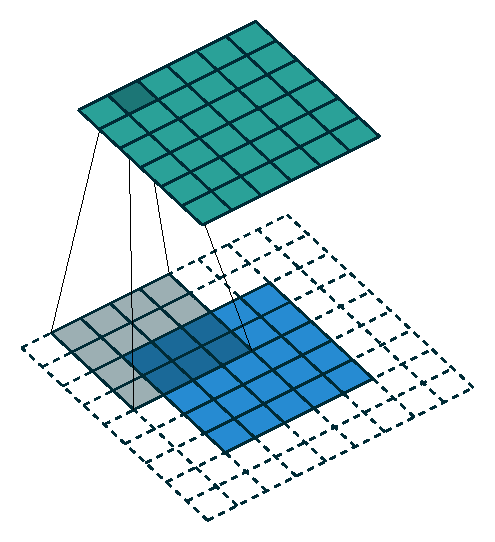
\includegraphics[width=0.6\linewidth]{images/arbitrary_padding_no_strides_01.pdf}
%    \label{fig:conv2d}
%\end{figure}

%\end{frame}


\begin{frame}{Background: Weight Pruning}

\begin{itemize}
    \item Pruning at the individual \textit{weight} level
    \item Leaves weight matrices very sparse
\end{itemize}

\begin{figure}
    \centering
    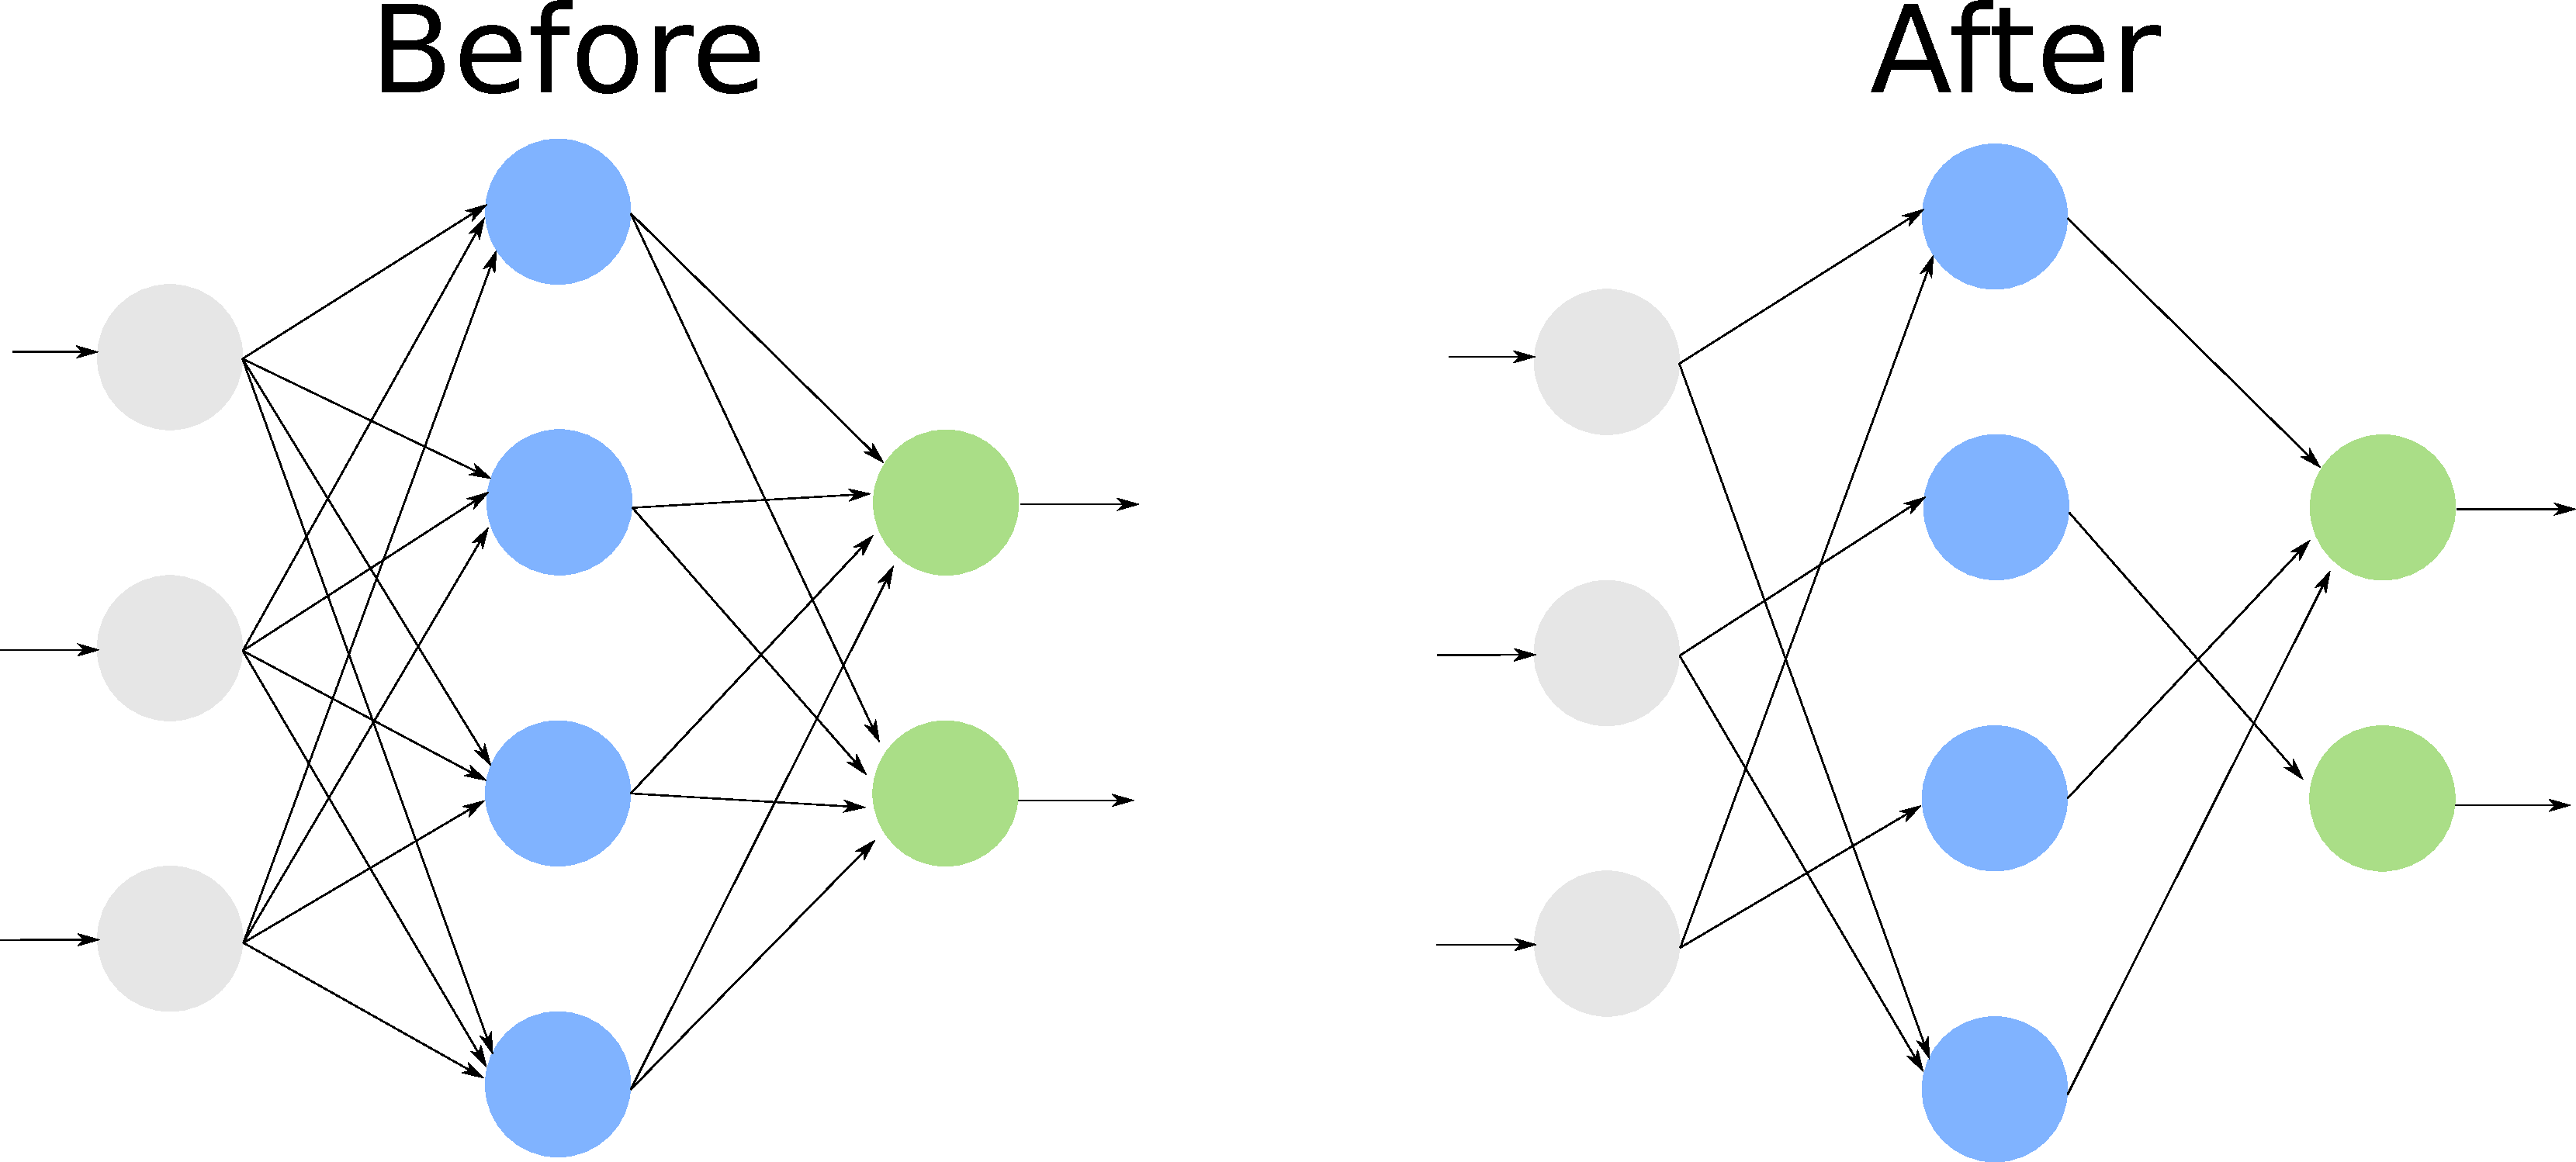
\includegraphics[width=8cm]{images/weight_pruning.pdf}
\end{figure}

\end{frame}


\begin{frame}{Background: Channel Pruning}

\begin{itemize}
    \item Pruning at the \textit{neuron} level
    \item Leaves weight matrices small and dense
\end{itemize}

\begin{figure}
    \centering
    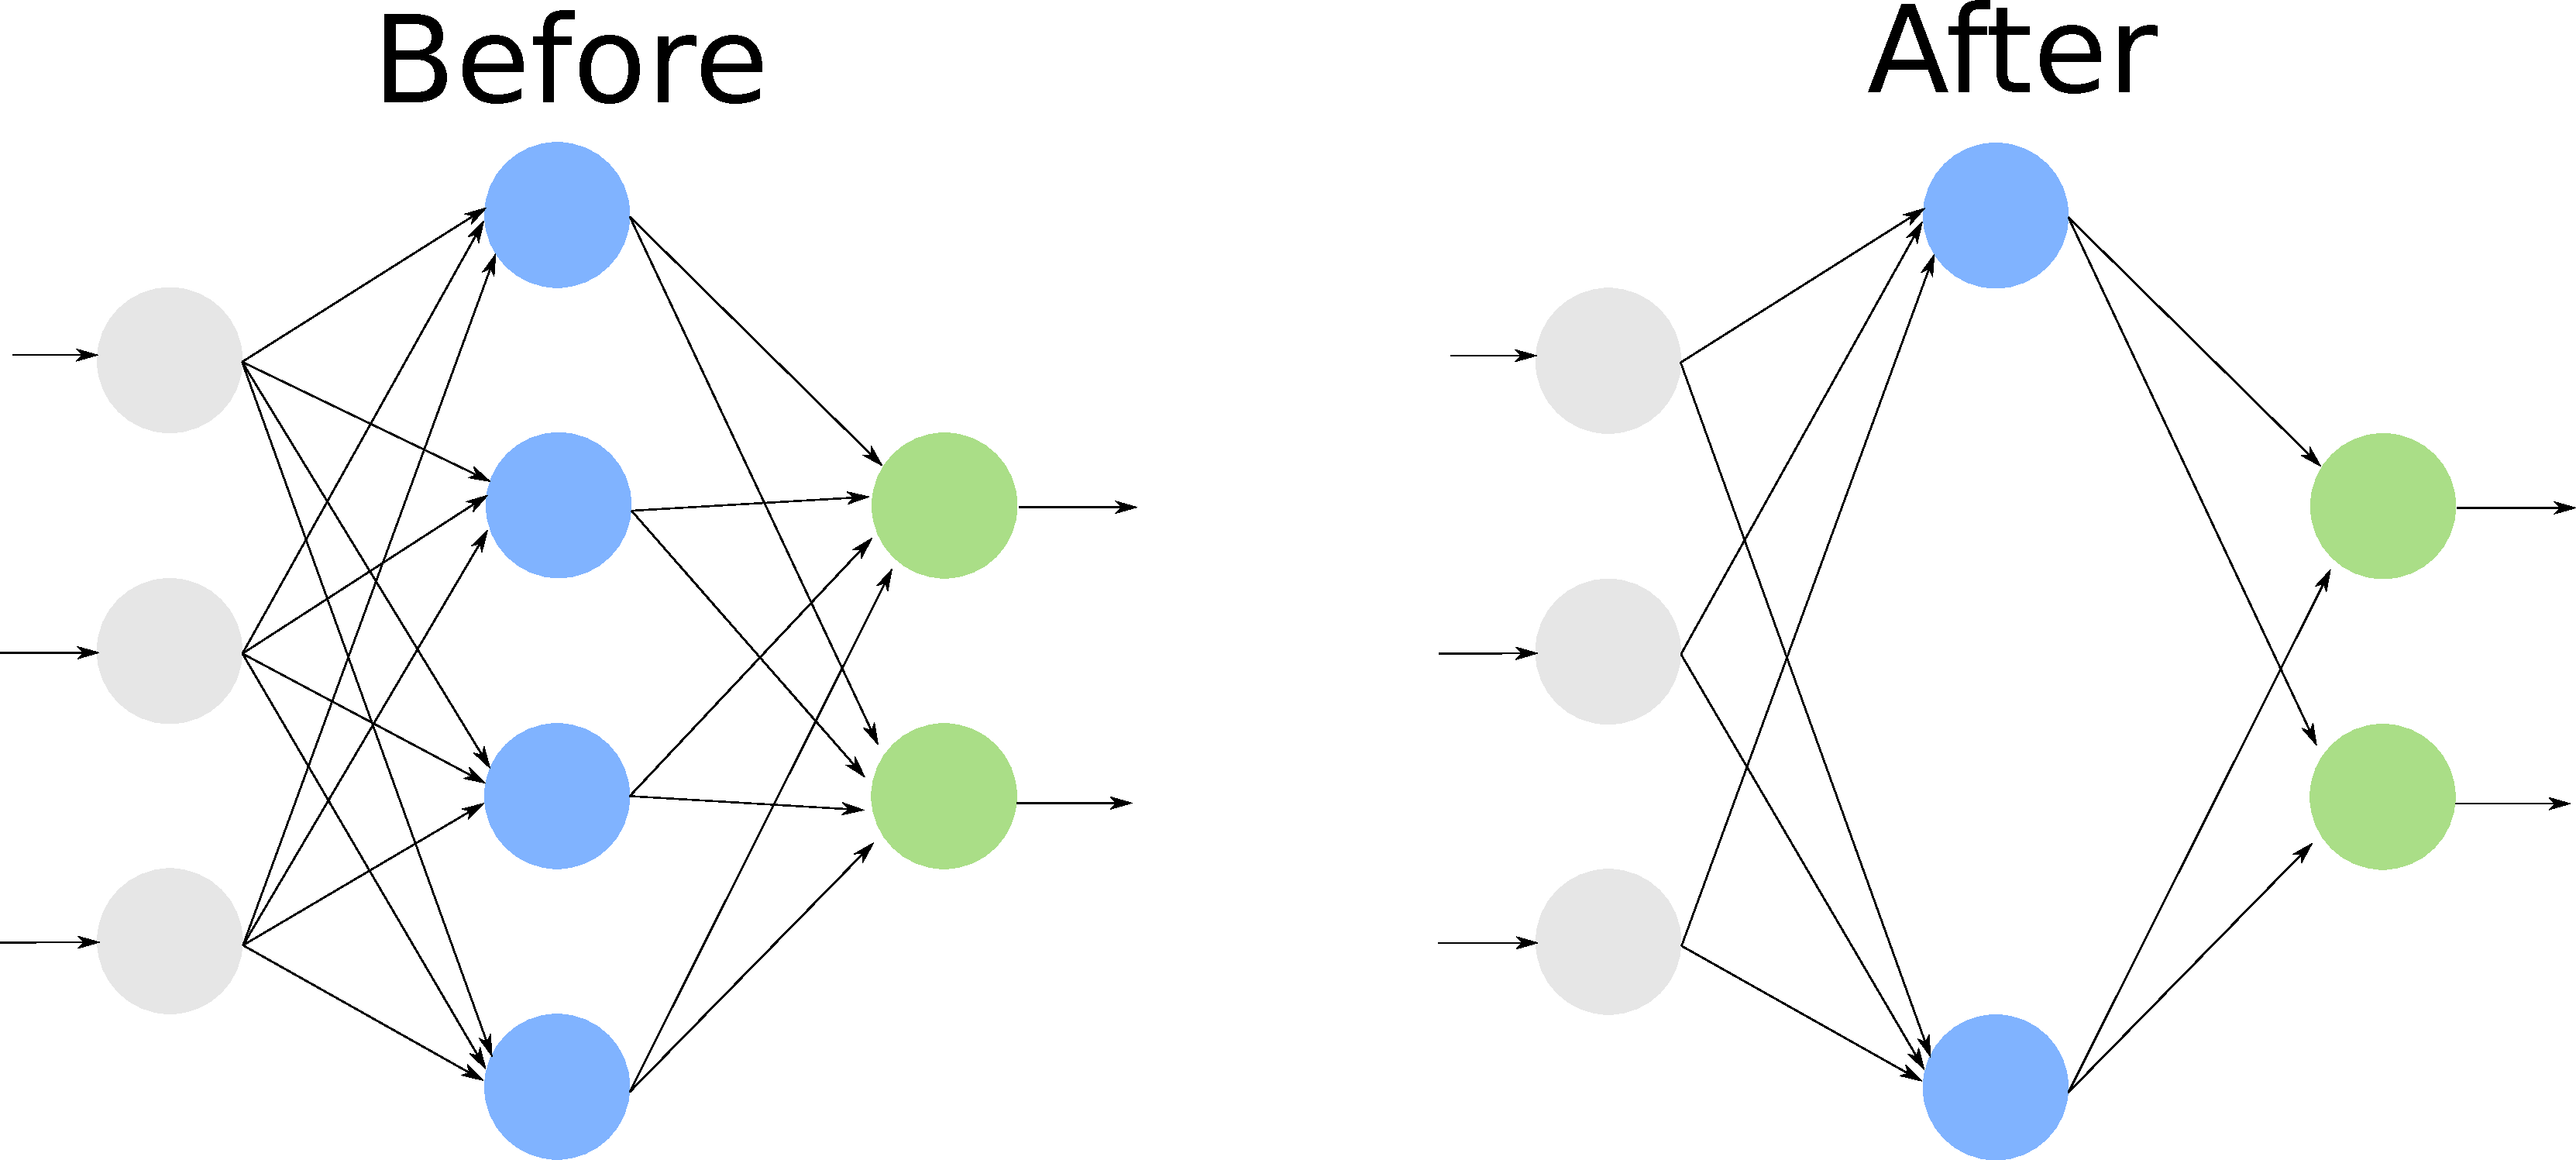
\includegraphics[width=8cm]{images/channel_pruning.pdf}
    \label{fig:channel_pruning}
\end{figure}

\end{frame}


\begin{frame}{Background: Quantisation}
\begin{itemize}
    \item Two options:
    \begin{enumerate}
        \item Reduce precision of weights
        \item \textbf{Group to small set of centroids}
    \end{enumerate}
\end{itemize}

\begin{figure}
    \centering
    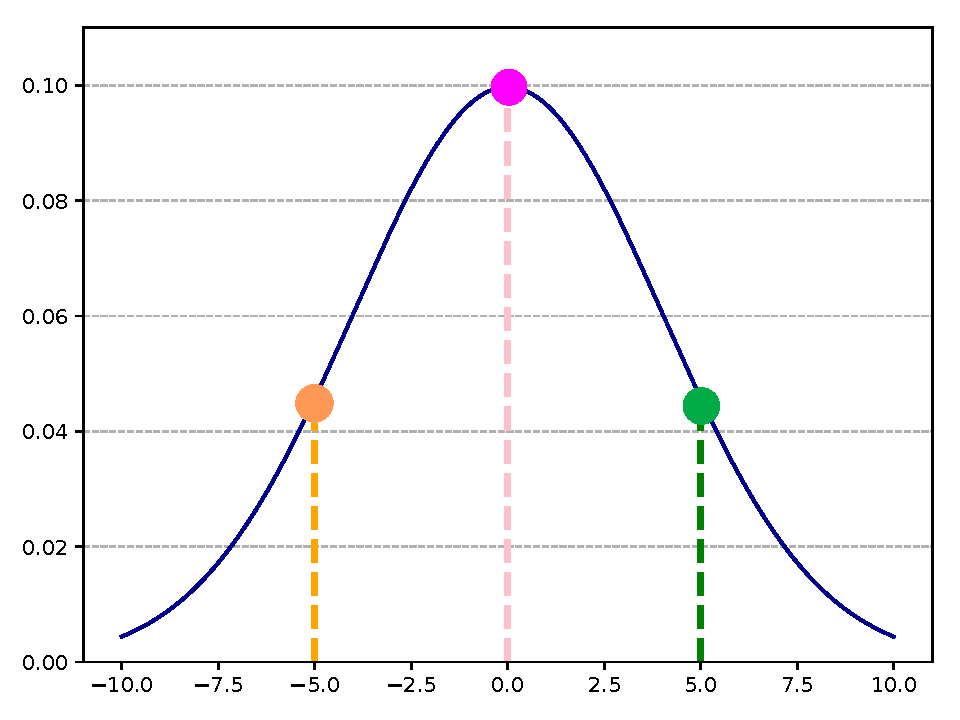
\includegraphics[width=5cm]{images/quantization.pdf}
\end{figure}


\end{frame}

\section{Inference Stack}

{
\setbeamercolor{background canvas}{bg=dark_blue!80}
\begin{frame}
    \centering
    \textcolor{white}{\LARGE Experimental methodology}
\end{frame}
}



\begin{frame}{CIFAR-10}

\begin{columns}
\column{0.5\textwidth}
\begin{figure}
    \centering
    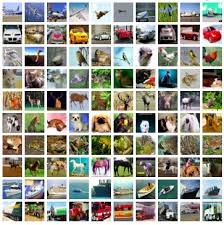
\includegraphics[width=\textwidth]{images/cifar.jpg}
\end{figure}

\column{0.5\textwidth}

\begin{itemize}
    \item $32 \times 32$ pixel images
    \item 10 classes
    \item 50,000 training images, 10,000 test images
\end{itemize}

\end{columns}
\end{frame}


\begin{frame}{Layer 1: Neural Networks}

\begin{columns}
\column{0.3\textwidth}

\begin{figure}
    \centering
    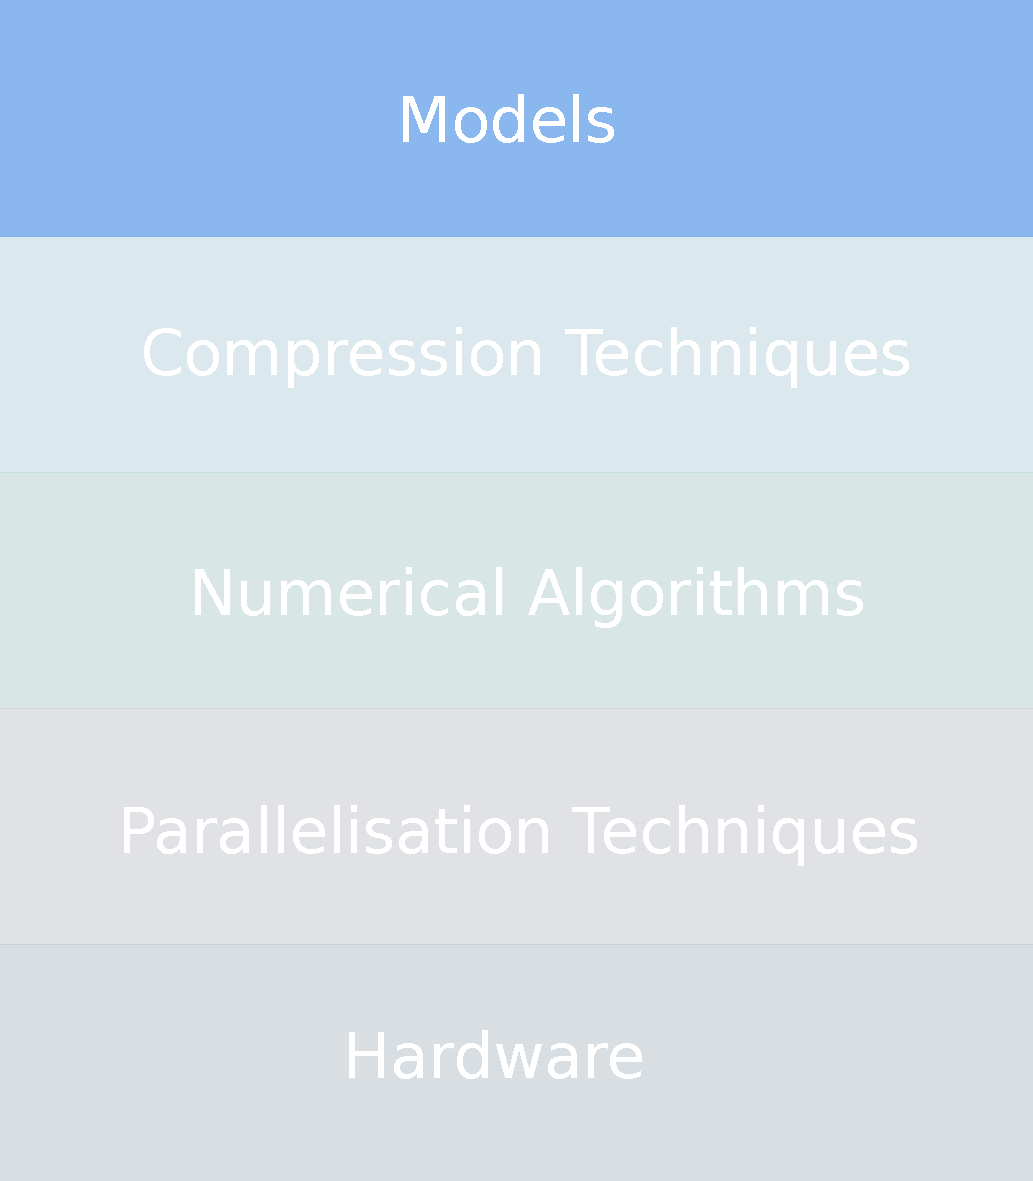
\includegraphics[width=3.5cm]{images/models.pdf}
    \label{fig:inference-stack-models}
\end{figure}

\column{0.7\textwidth}

\textbf{Neural Network Models}


\begin{table}[]
    \centering
    \begin{tabular}{c|c|c}
        Model & Accuracy & Weight size \\
        \hline
        VGG-16 & 92.0\% & 309.1 MB \\
        MobileNet & 91.5\% & \textbf{66.3 MB}\\
        ResNet-18 & \textbf{94.2\%} & 233.8 MB \\
    \end{tabular}
\end{table}

\end{columns}


\end{frame}

\definecolor{bg}{rgb}{0.95,0.95,0.95}

%\begin{frame}{Layer 1: Neural Networks}
%\vspace{0.2cm}

%\inputminted[bgcolor=bg, fontfamily=cmss]{python}{images/mini_model.py}

%\begin{figure}
%    \centering
%    \vspace{-1cm}
%    
\includegraphics[width=10cm]{images/lgoos.pdf}
%\end{figure}
%\end{frame}


%\begin{frame}{Layer 1: Neural Networks}
%\vspace{0.2cm}

%\begin{figure}
%    \centering
%    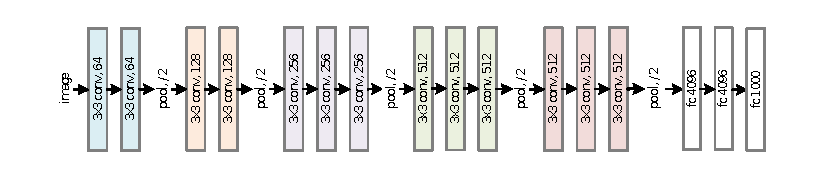
\includegraphics[width=0.8\linewidth]{images/vgg.pdf}
%    \caption{VGG-16}
%\end{figure}


%\begin{figure}
%    \centering
%    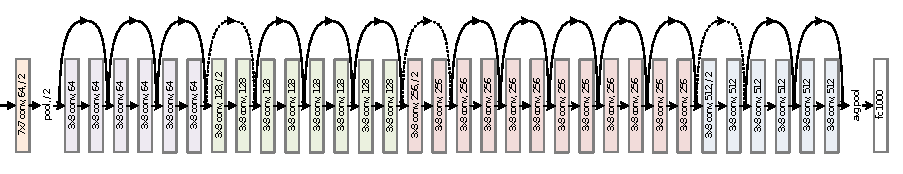
\includegraphics[width=0.8\linewidth]{images/resnet.pdf}
%    \caption{ResNet-18}
%\end{figure}

%{\color{red} MobileNet figure goes here}

%\end{frame}


\begin{frame}{Layer 2: Compression Techniques}

\begin{columns}
\column{0.3\textwidth}
\begin{figure}
    \centering
    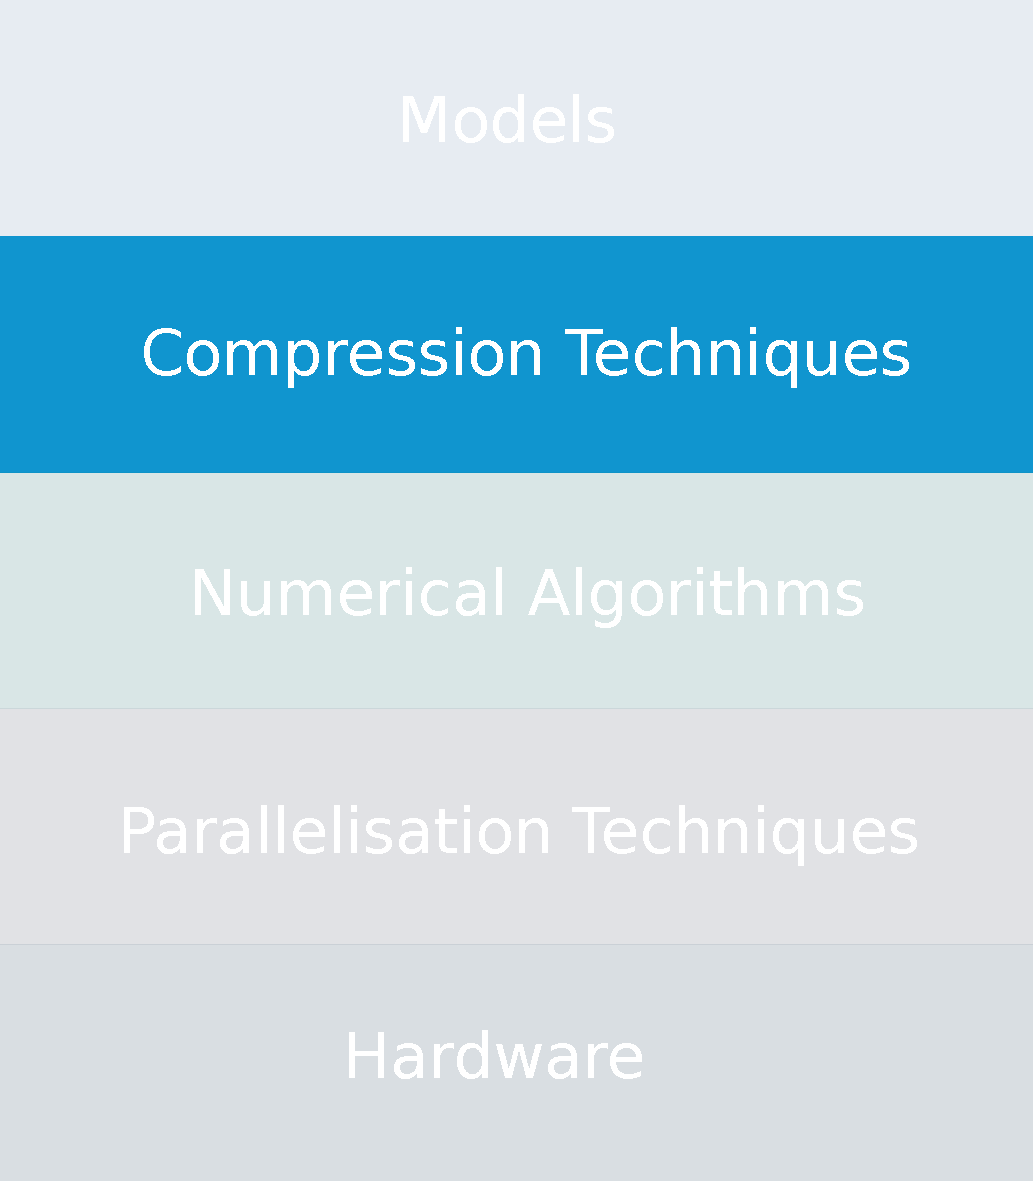
\includegraphics[width=3.5cm]{images/compressions.pdf}
    \label{fig:inference-stack-compress-1}
\end{figure}

\column{0.7\textwidth}
We consider representatives from three different classes of compression technique:
\begin{enumerate}
    \item Weight Pruning
    \item Channel Pruning
    \item Quantisation
\end{enumerate}


\end{columns}

\end{frame}



\begin{frame}{Layer 2: Weight Pruning}

{\large\textbf{General Idea}}

\begin{itemize}
    \item Magnitude based thresholding 
    \item Iterate over steps of sparsifying and retraining 
    \item Leave the matrices very sparse but get up to 90\% compression rate
\end{itemize}

\begin{figure}
    \centering
    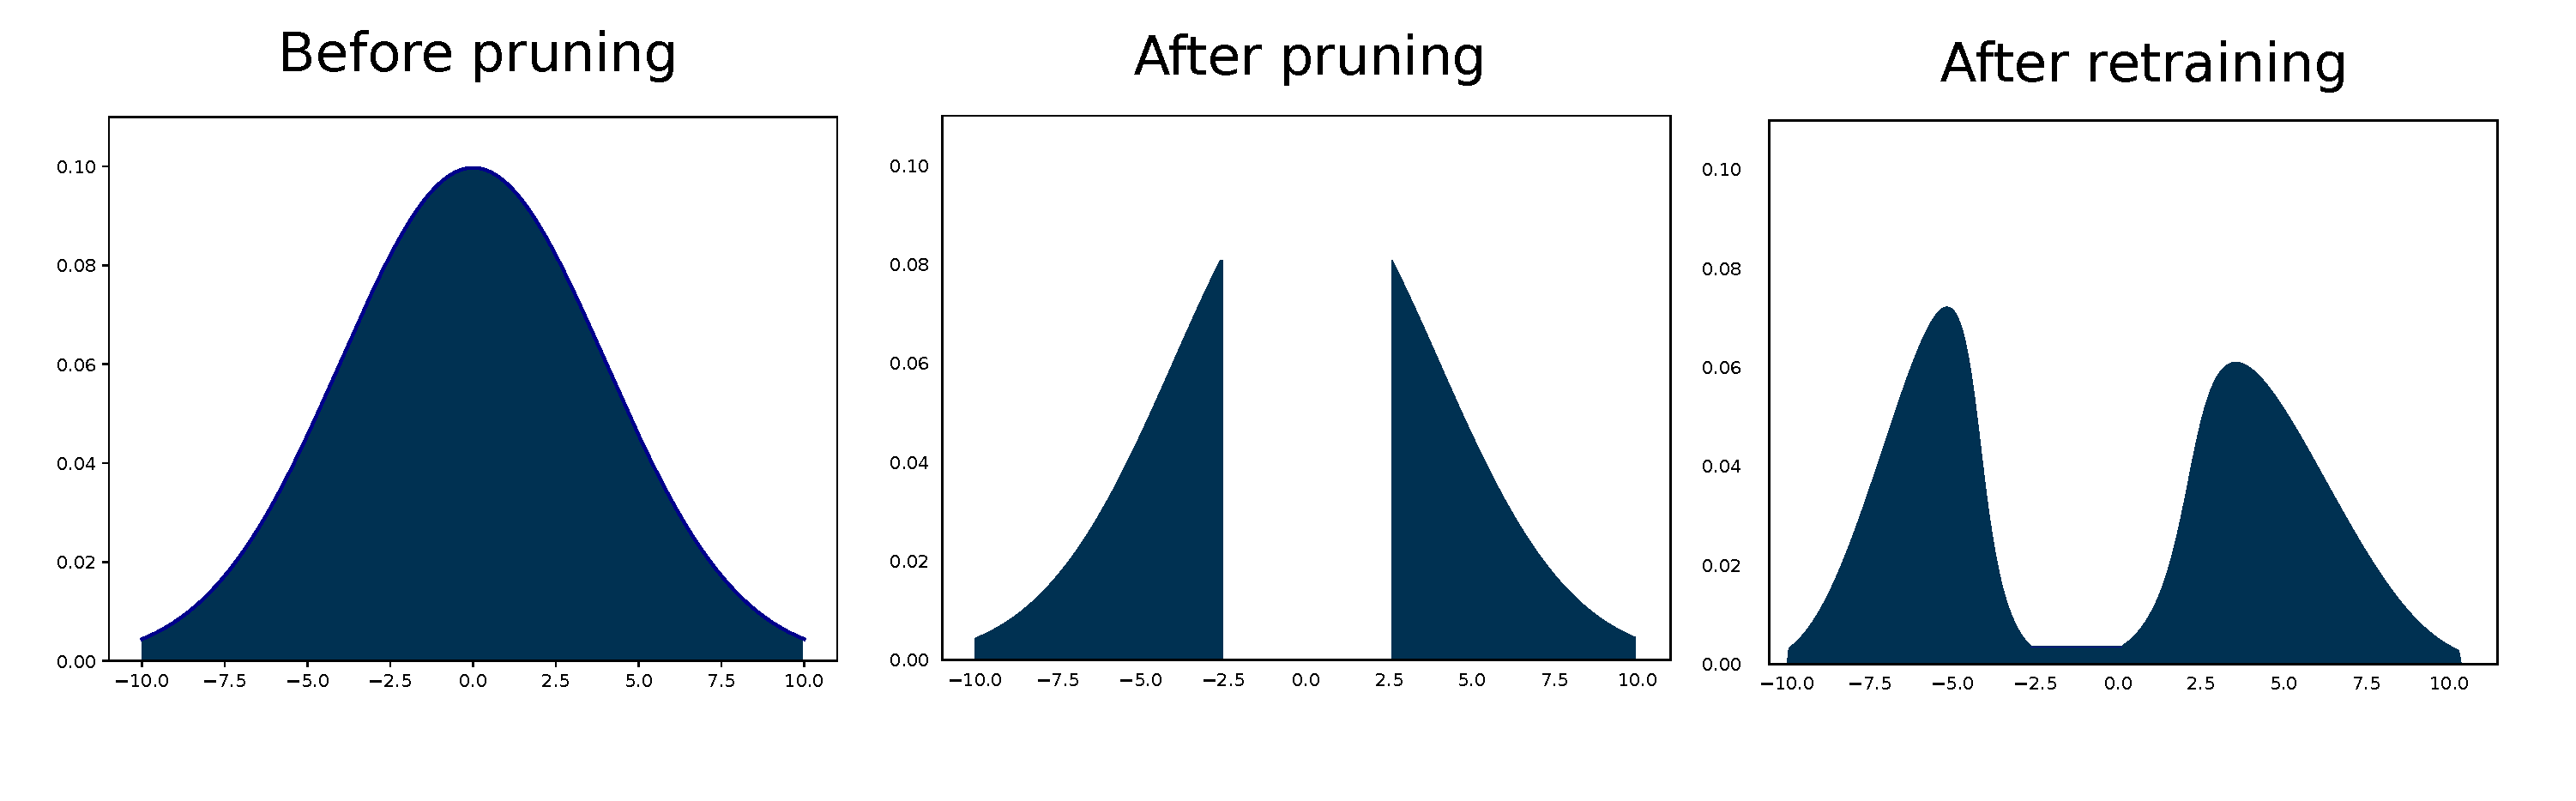
\includegraphics[width=\linewidth]{images/prune_retrain.pdf}
\end{figure}

{\footnotesize [Han, S., Mao, H. and Dally, W.J., 2015. Deep Compression]}
    
\end{frame}


\begin{frame}{Layer 2: Channel Pruning}
    
{\large\textbf{General Idea}}
\begin{itemize}
    \item Use second-order Taylor expansion of error function to estimate effect of removing neuron \textit{n}
    \item Weight with a FLOP penalty $\beta$ to bias towards removing expensive neurons
    \item Iteratively remove neurons and retrain
\end{itemize}

%If we are optimising the parameters $\theta$ for some error function $\mathcal{L}$, then removing parameter $\theta_{k}$ will change the error by:
%\begin{equation}
%    \mathcal{L}(\theta - \theta_{ke_{k}}) - \mathcal{L}(\theta) = -g_{k}\theta_{k} + \frac{1}{2}H_{kk}\theta^2_{k}
%\end{equation}

\vspace{2cm}

{\footnotesize [Theis et. al, 2018. Faster gaze prediction with dense networks and Fisher pruning.]}
    
\end{frame}


\begin{frame}{Layer 2: Quantisation}


{\large\textbf{General Idea}}
\begin{itemize}
    \item Set three centroid values and group all of the weights to each centroid
    \item Inference can be done with just these three values
    \item Often also have some sparsity (since one of the three values is usually zero)
\end{itemize}

\begin{figure}
    \centering
    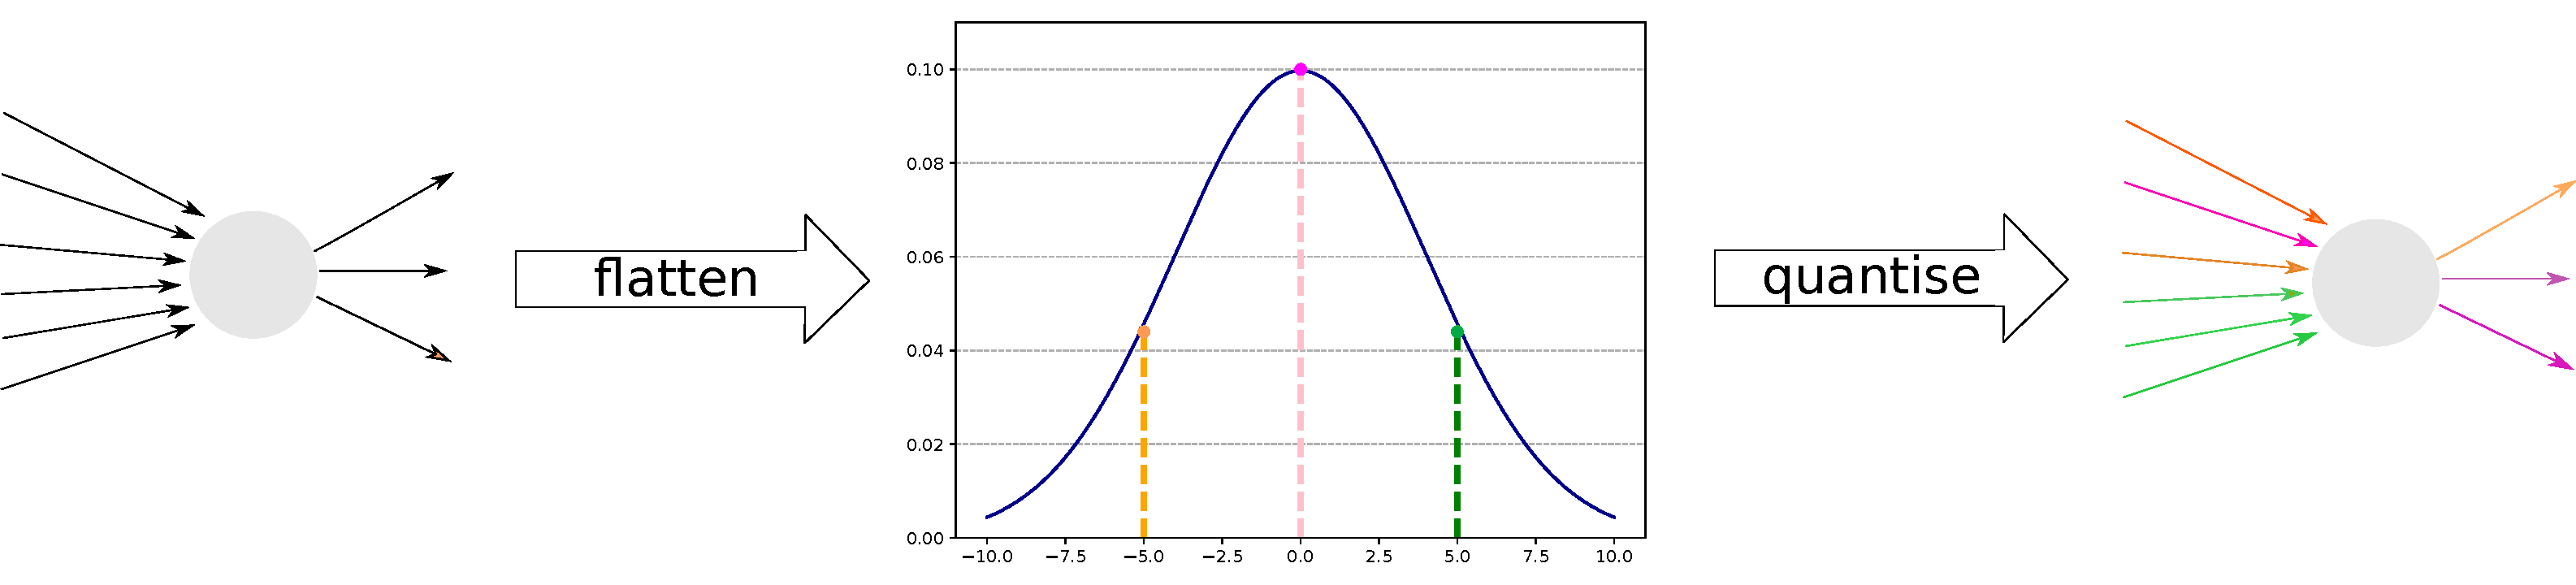
\includegraphics[width=\linewidth]{images/quantization_pipeline.pdf}
\end{figure}
    
{\footnotesize [Zhu et. al, 2017. Trained Ternary Quantization.]}    

\end{frame}


\begin{frame}

\begin{figure}
    \centering
    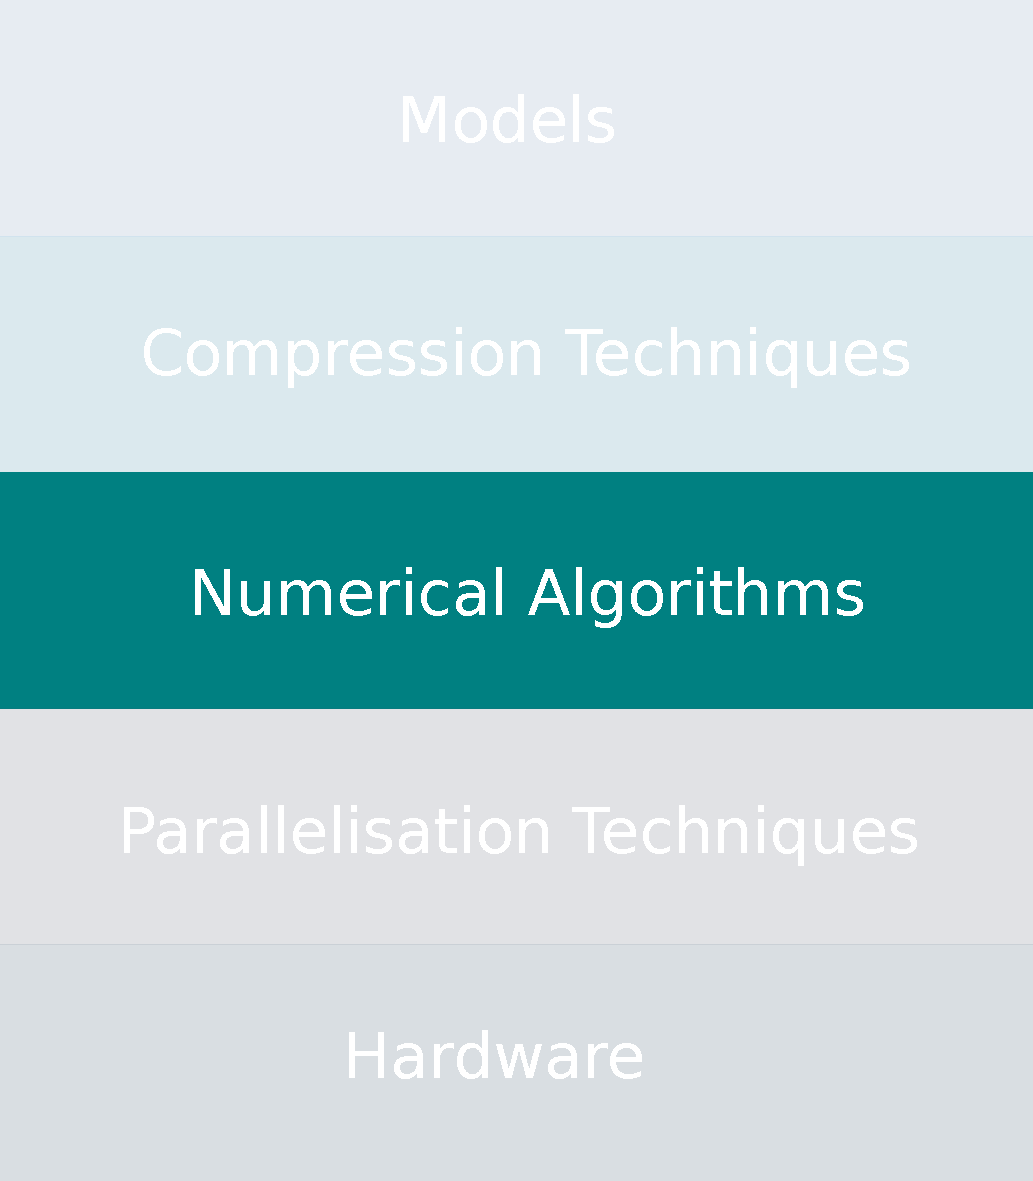
\includegraphics[width=0.6\linewidth]{images/numericals.pdf}
\end{figure}
    
\end{frame}

\begin{frame}{Layer 3: Numerical Algorithms}

\begin{columns}

\column{0.3\textwidth}
\begin{figure}
    \centering
    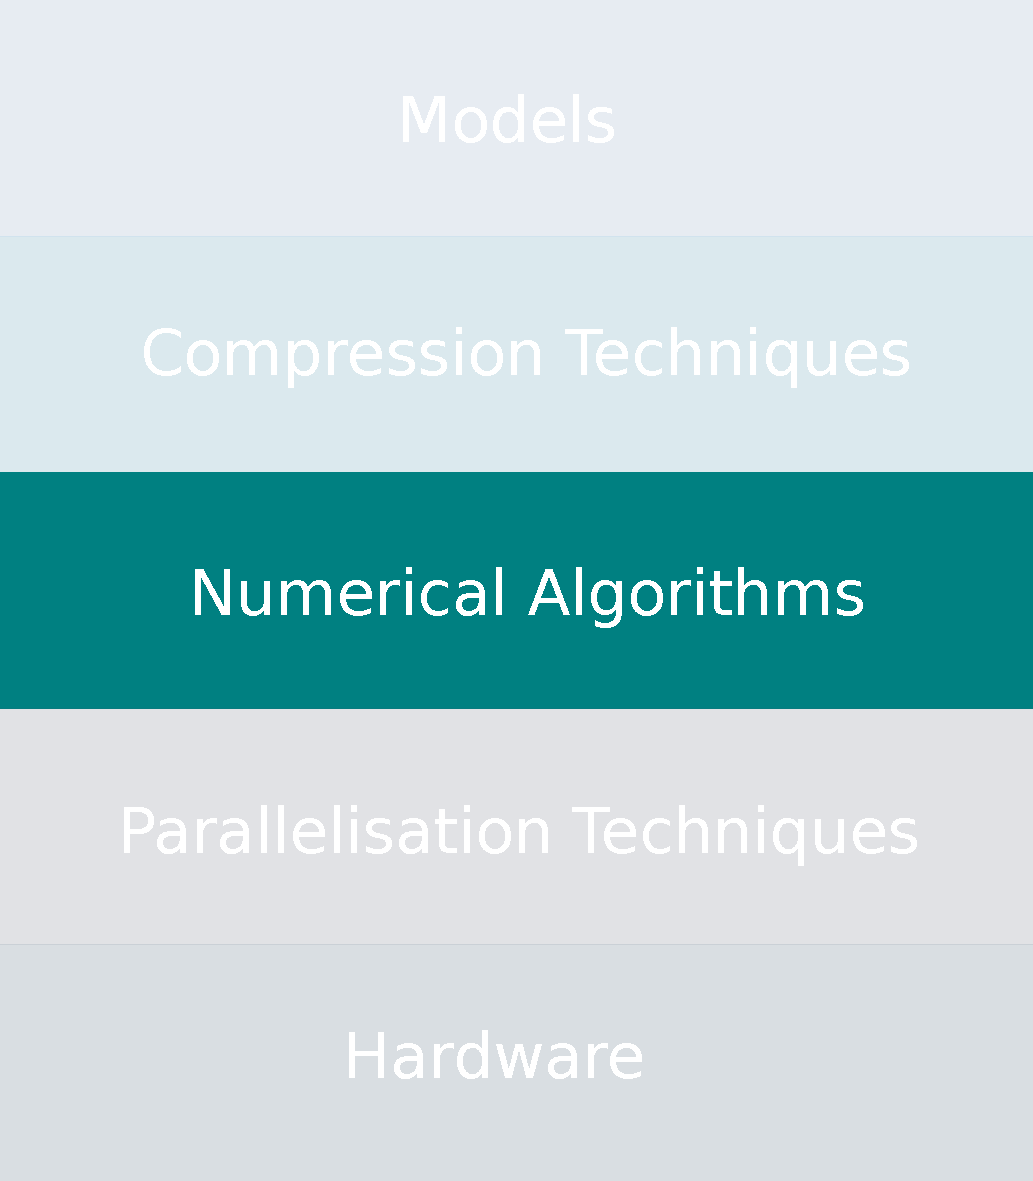
\includegraphics[width=3.5cm]{images/numericals.pdf}
    \label{fig:inference-stack-nums-1}
\end{figure}

\column{0.7\textwidth}

{\large Direct Convolution\footnotemark}

\begin{figure}
    \centering
    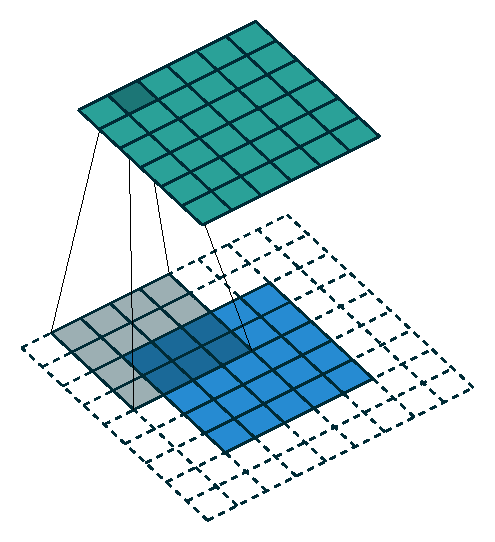
\includegraphics[width=5cm]{images/arbitrary_padding_no_strides_01.pdf}
\end{figure}

\end{columns}

\footnotetext{https://github.com/vdumoulin/conv\_arithmetic}

\end{frame}

\begin{frame}{Layer 3: Numerical Algorithms}

\begin{columns}

\column{0.3\textwidth}
\begin{figure}
    \centering
    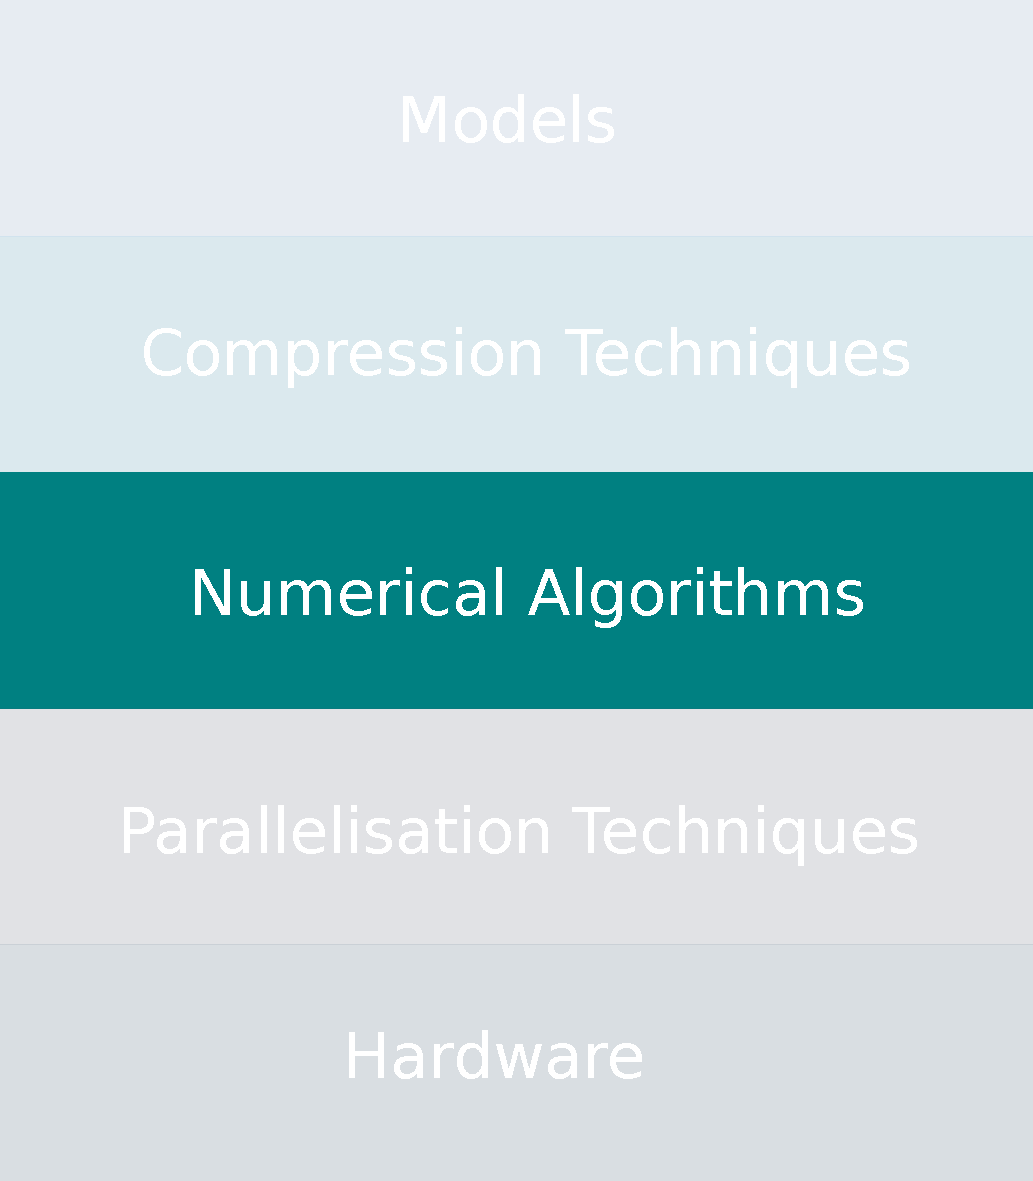
\includegraphics[width=3.5cm]{images/numericals.pdf}
    \label{fig:inference-stack-nums-2}
\end{figure}

\column{0.7\textwidth}

{\large Convolution as SGEMM \footnotemark}

\begin{figure}
    \centering
    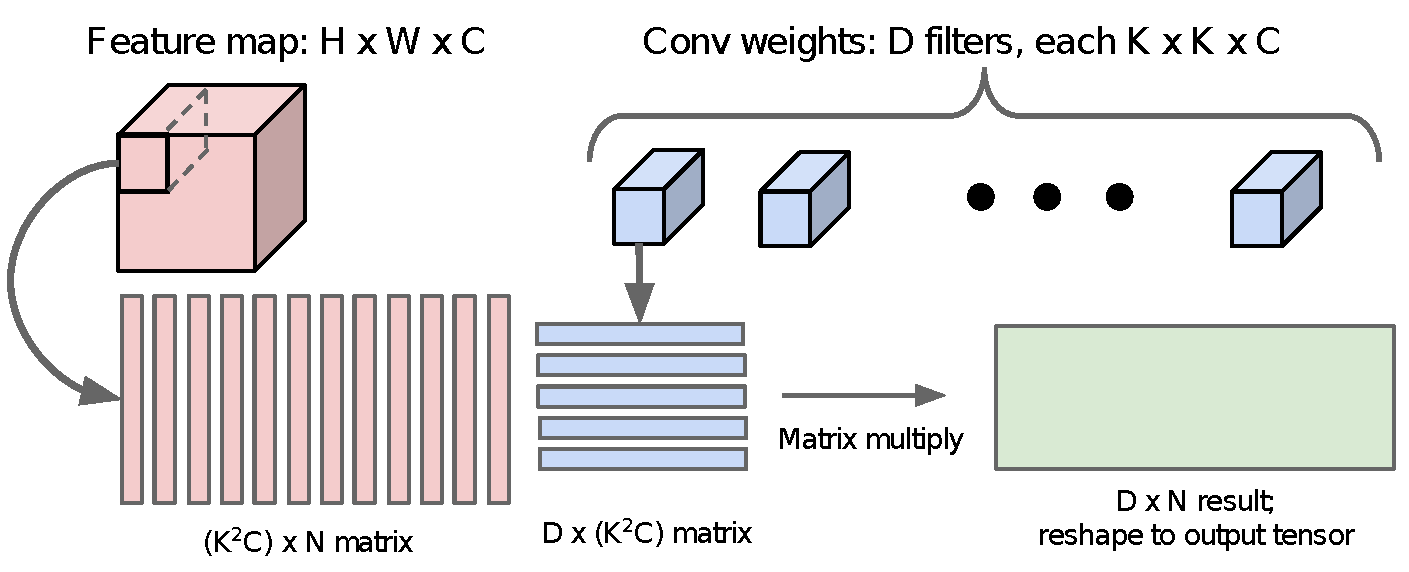
\includegraphics[width=8cm]{images/im2col.pdf}
\end{figure}

\end{columns}

\footnotetext{http://cs231n.stanford.edu/slides/2016/winter1516\_lecture11.pdf}
\end{frame}


\begin{frame}{Compressed Sparse Row (CSR) Format}

\begin{columns}

\column{0.3\textwidth}

\begin{figure}
    \centering
    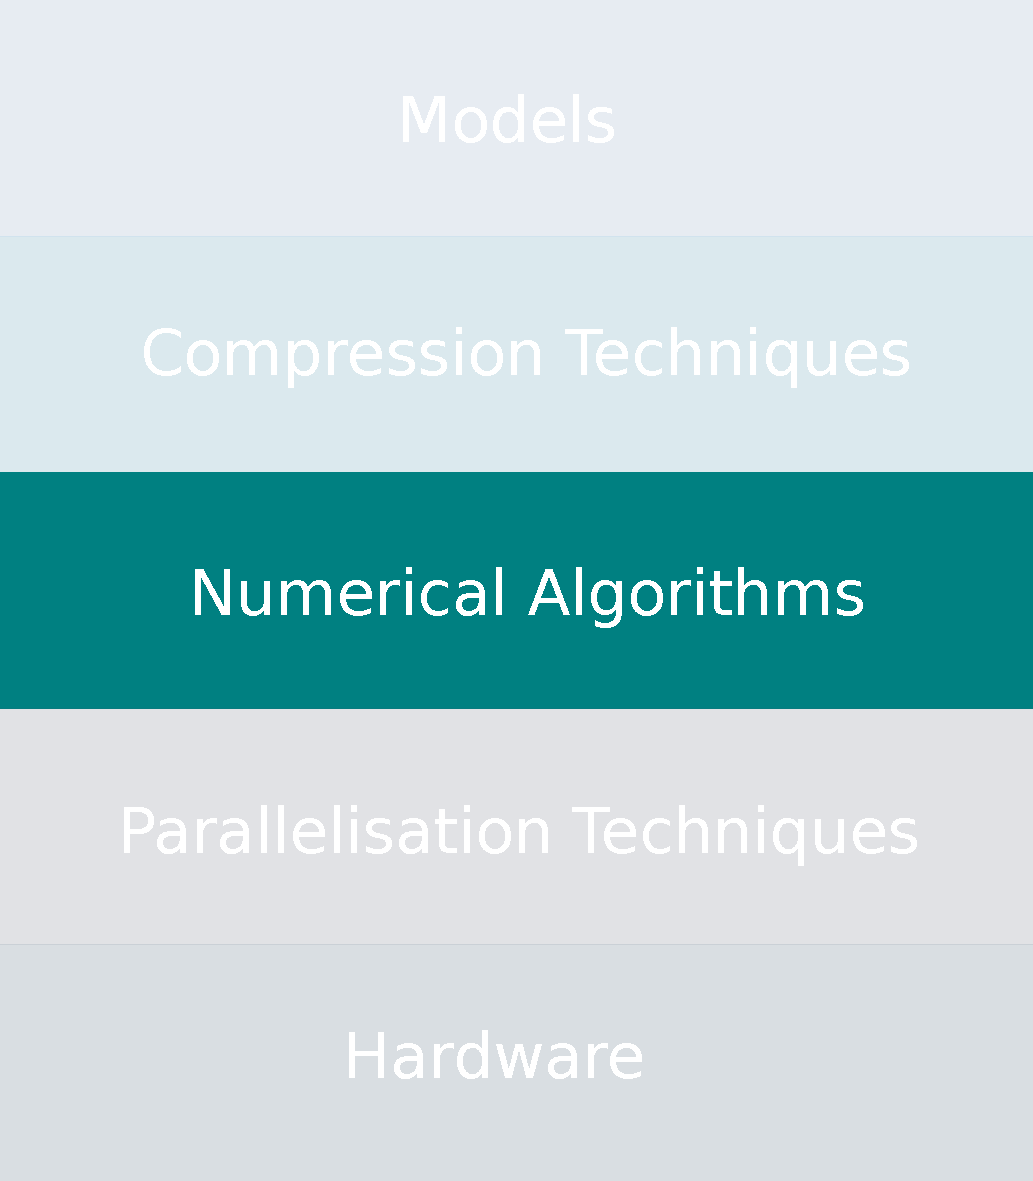
\includegraphics[width=3.5cm]{images/numericals.pdf}
    \label{fig:inference-stack-nums-3}
\end{figure}

\column{0.7\textwidth}
When the matrices are very sparse, we may wish to use a sparse representation format: 

\begin{figure}
    \centering
    \includegraphics[width=\linewidth]{images/CSR.pdf}
\end{figure}

\end{columns}
\end{frame}

\begin{frame}

\begin{figure}
    \centering
    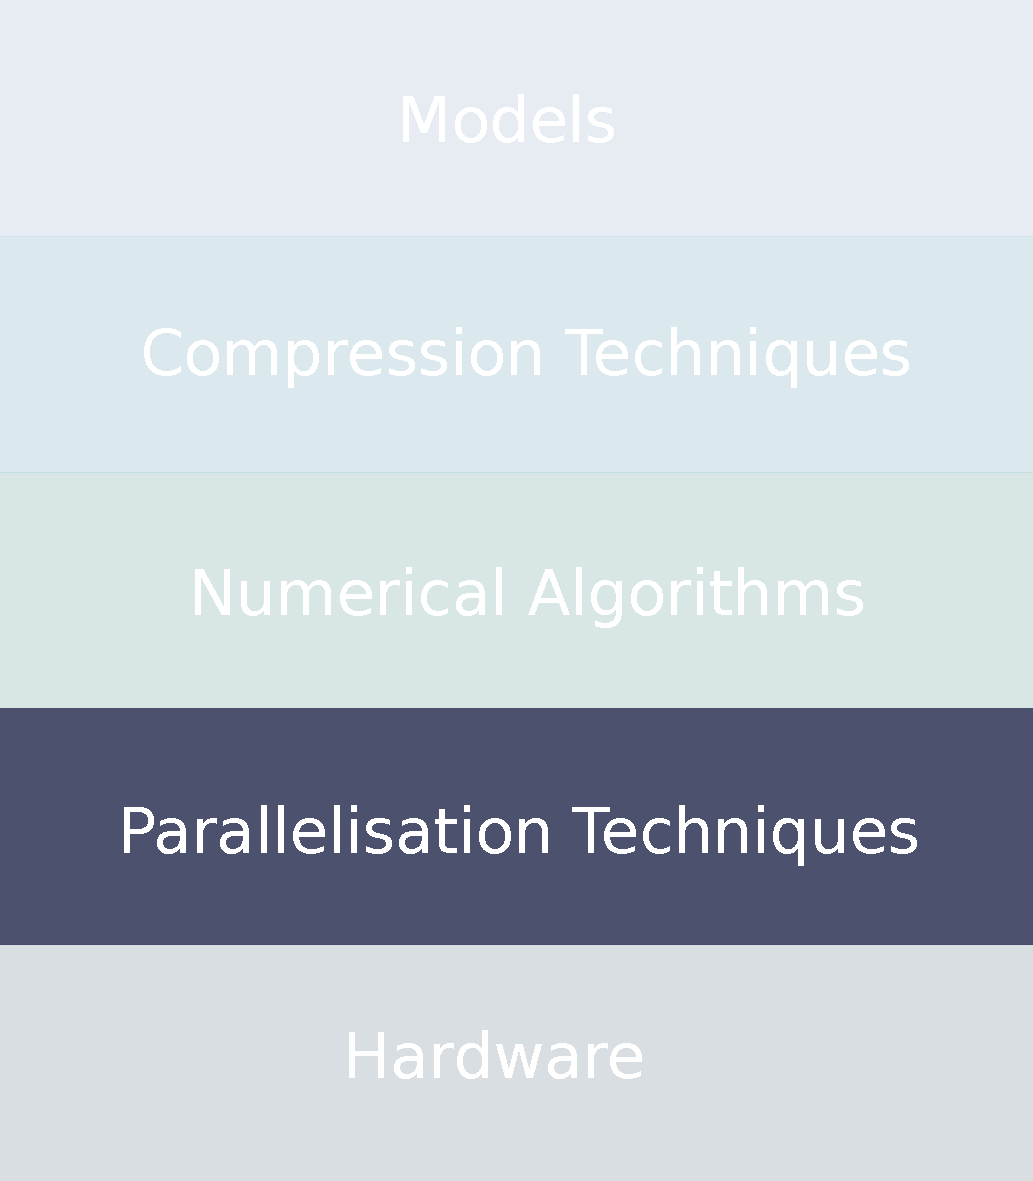
\includegraphics[width=0.6\linewidth]{images/parallelisations.pdf}
\end{figure}
\end{frame}


\begin{frame}[fragile]{OpenMP Parallelisation}

\begin{lstlisting}[language=C, columns=fullflexible]
#pragma omp parallel for schedule(dynamic,1) num_threads(t)
for (i = 0; i < out_planes; i++) {
	for (j = 0; j < in_planes; j++) {
		convolution_3_x_3(inputs[j], weights[layer][i][j]);
	}
}
\end{lstlisting}


\end{frame}



\begin{frame}{Layer 4: Parallelisation Techniques}

\begin{columns}


\column{0.3\textwidth}
\begin{figure}
    \centering
    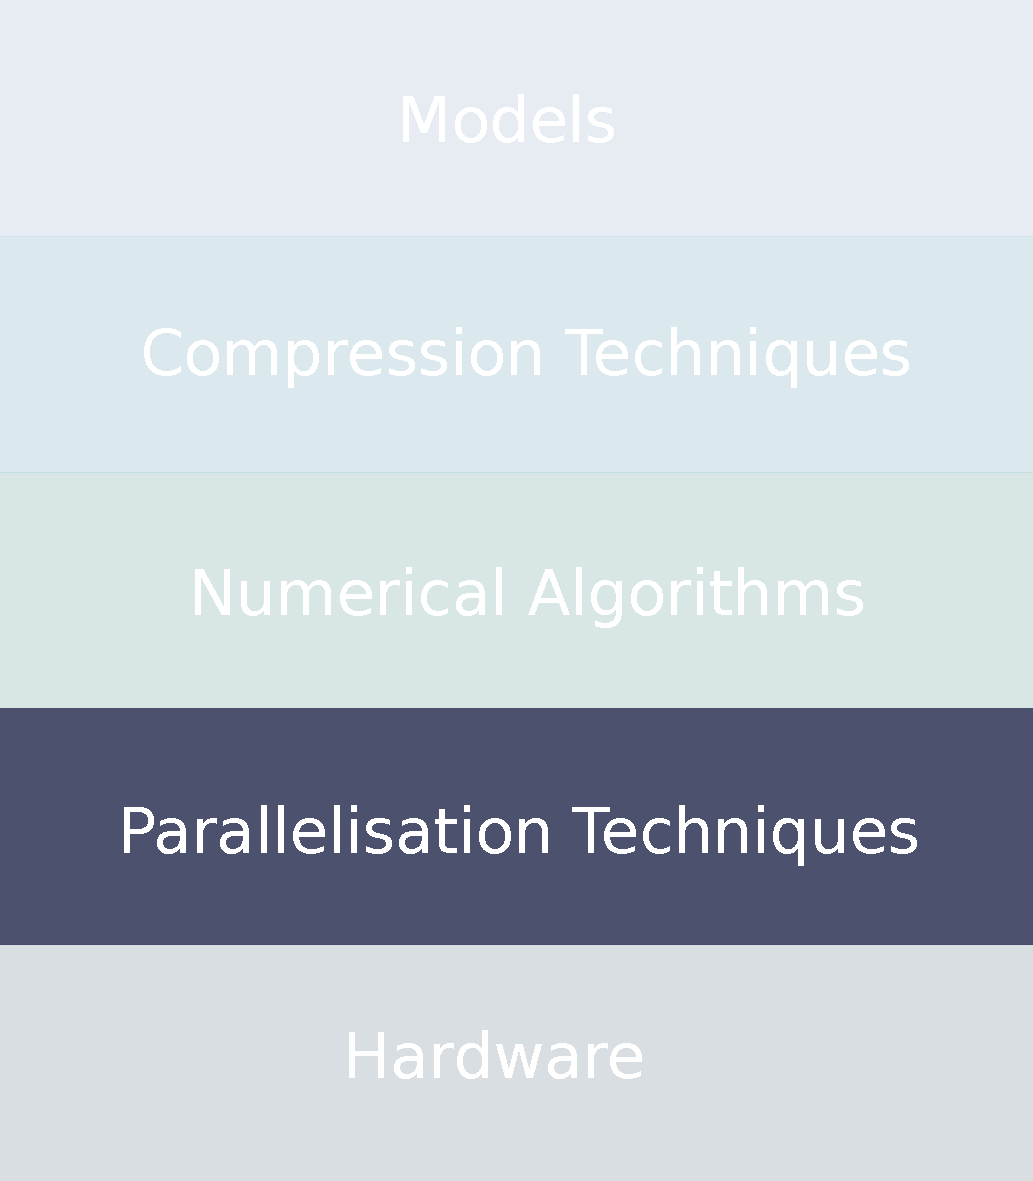
\includegraphics[width=3.5cm]{images/parallelisations.pdf}
    \label{fig:inference-stack-parallels-2}
\end{figure}

\column{0.7\textwidth}

\textbf{OpenCL}
\begin{itemize}
    \item Hand tuned work groups, tiling and register blocking
    \item CLBlast Autotuning 
\end{itemize}

\end{columns}

\end{frame}

\begin{frame}

\begin{figure}
    \centering
    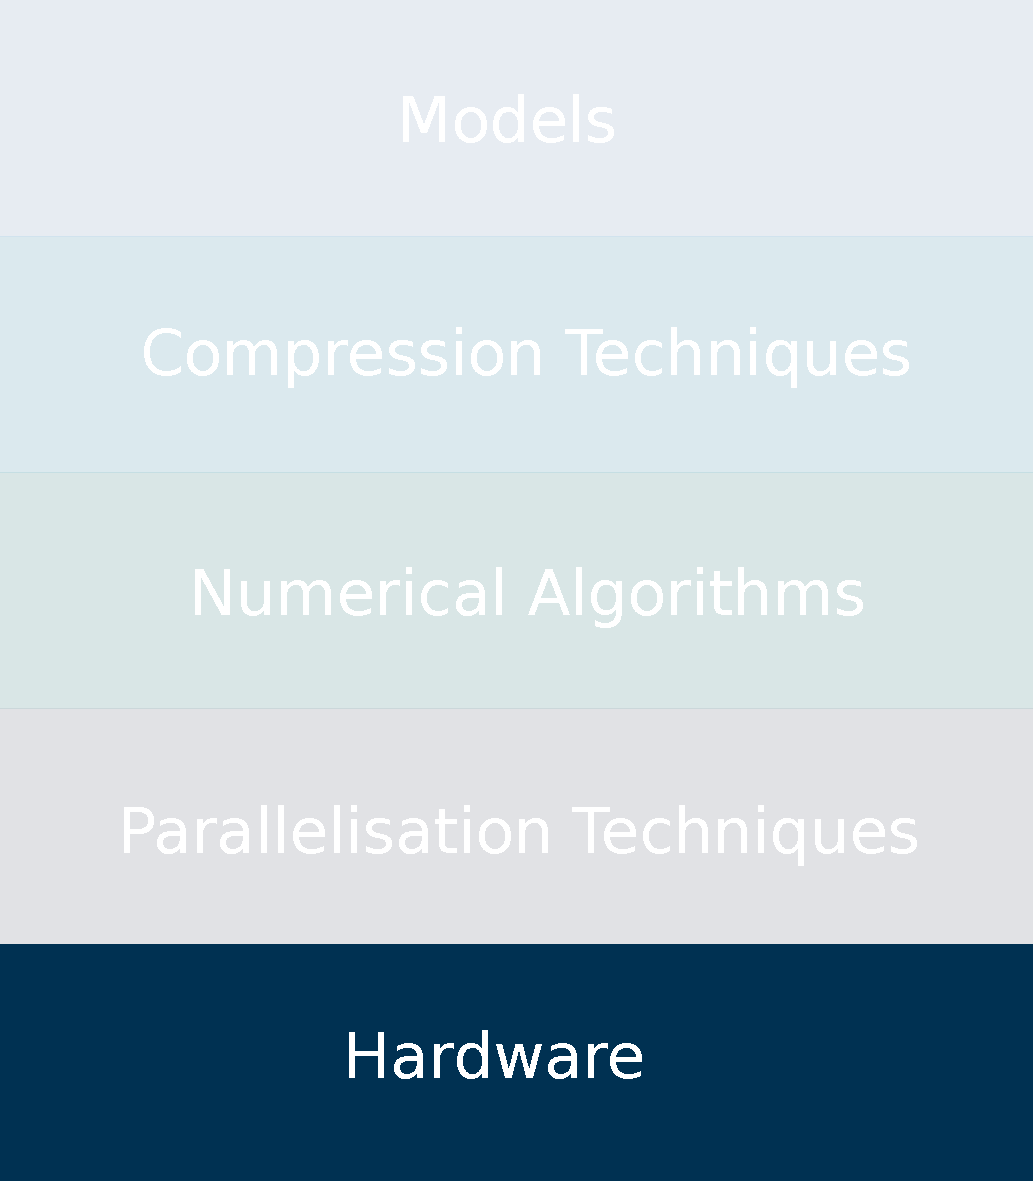
\includegraphics[width=0.6\linewidth]{images/hardwares.pdf}
\end{figure}
\end{frame}

\begin{frame}{Layer 5: Hardware}

\begin{columns}


\column{0.3\textwidth}
\begin{figure}
    \centering
    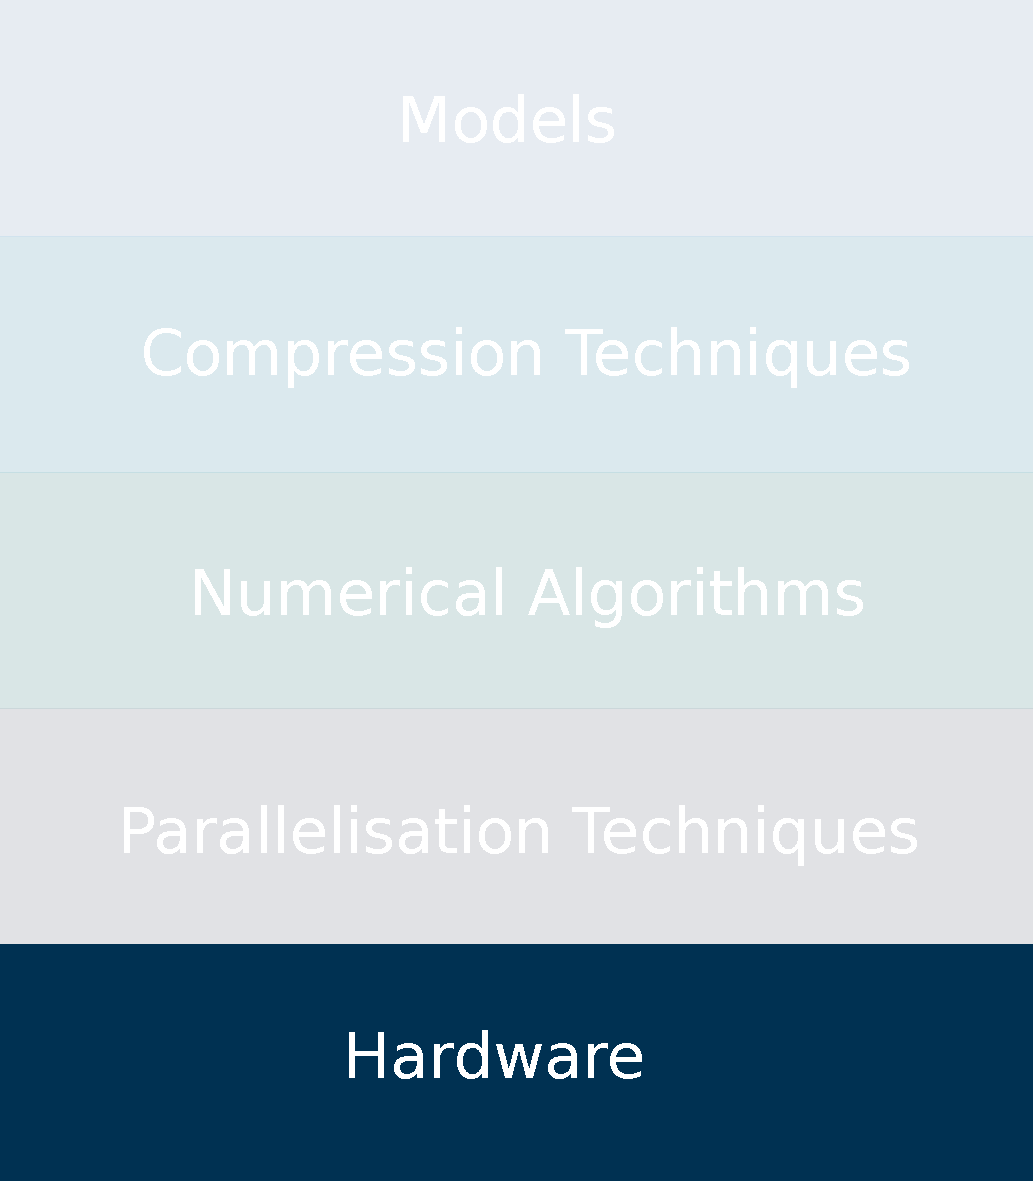
\includegraphics[width=3.5cm]{images/hardwares.pdf}
\end{figure}

\column{0.7\textwidth}

Desktop compute:
\begin{itemize}
    \item Intel Core i7 (4 cores) w. 8GB RAM
\end{itemize}

\vspace{0.5cm}
Embedded heterogeneous hardware:
\begin{itemize}
    \item Odroid-XU4 (ARM big.LITTLE CPU (8 cores) + Mali T628 GPU (6 cores) w. 2GB RAM
\end{itemize}
\end{columns}


\end{frame}




\section{Experiments}

{
\setbeamercolor{background canvas}{bg=dark_blue!80}
\begin{frame}
    \centering
    \textcolor{white}{\LARGE Experiments}
\end{frame}
}

\begin{frame}{Impact of Compression on Accuracy}

\begin{itemize}
    \item Quantisation performs particularly badly on MobileNet
    \item Channel pruning $>$ weight pruning
\end{itemize}
    
\vspace{0.5cm}
\begin{figure}
    \centering
    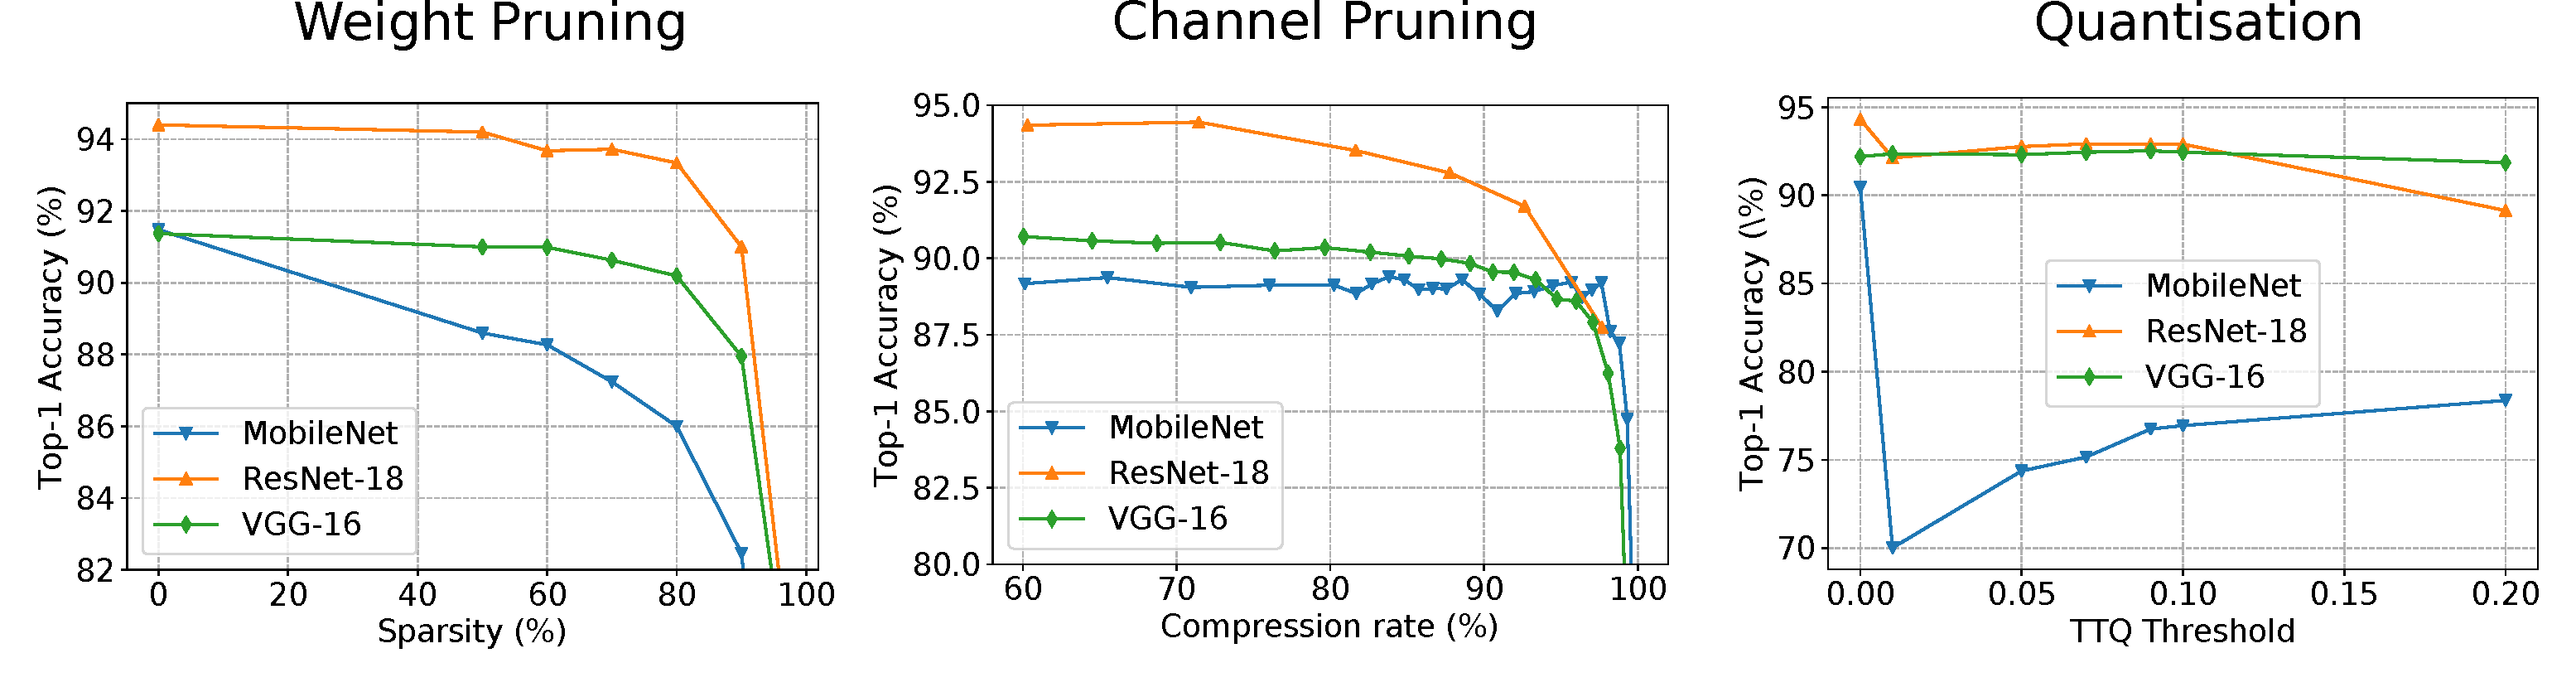
\includegraphics[width=1.08\linewidth]{images/accuracies.pdf}
\end{figure}
    
\end{frame}

\begin{frame}{Impact of Compression on Memory Footprint}
    
\begin{table}[h]
\begin{center}

%\vspace{-0.2cm}
\begin{tabular}{ |c|c|c|c|c| } \hline
Model&Plain&W. Pruning &C.~Pruning&T. Quantis.\\ \hline \hline
VGG-16 	  &	309.9	& 112.2	& 74.9	& 114.1 \\ \hline
ResNet-18 &	233.8	& 66.1	& {\color{red}\textbf{13.1}}	& 66.9 \\ \hline
MobileNet & {\color{red}\textbf{66.3}} & 40.9	& 2.7	& 63.3 \\ \hline
\end{tabular}
%\vspace{-0.8cm}
\label{table:mem-90}
\end{center}
\end{table}

\end{frame}

\begin{frame}{Impact of Compression on Memory Footprint}
    
\begin{table}[h]
\begin{center}

%\vspace{-0.2cm}
\begin{tabular}{ |c|c|c|c|c| } \hline
Model&Plain&W. Pruning &C.~Pruning&T. Quantis.\\ \hline \hline
VGG-16 	  &	309.9	& 112.2	& 74.9	& 114.1 \\ \hline
ResNet-18 &	233.8	& 66.1	& 13.1	& 66.9 \\ \hline
MobileNet & 66.3 & 40.9	& {\color{red}\textbf{2.7}}	& 63.3 \\ \hline
\end{tabular}
%\vspace{-0.8cm}
\label{table:mem-90}
\end{center}
\end{table}

\end{frame}


\begin{frame}{Impact of Compression on Inference Speed}
    
    VGG-16:
    
    \begin{figure}
        \centering
        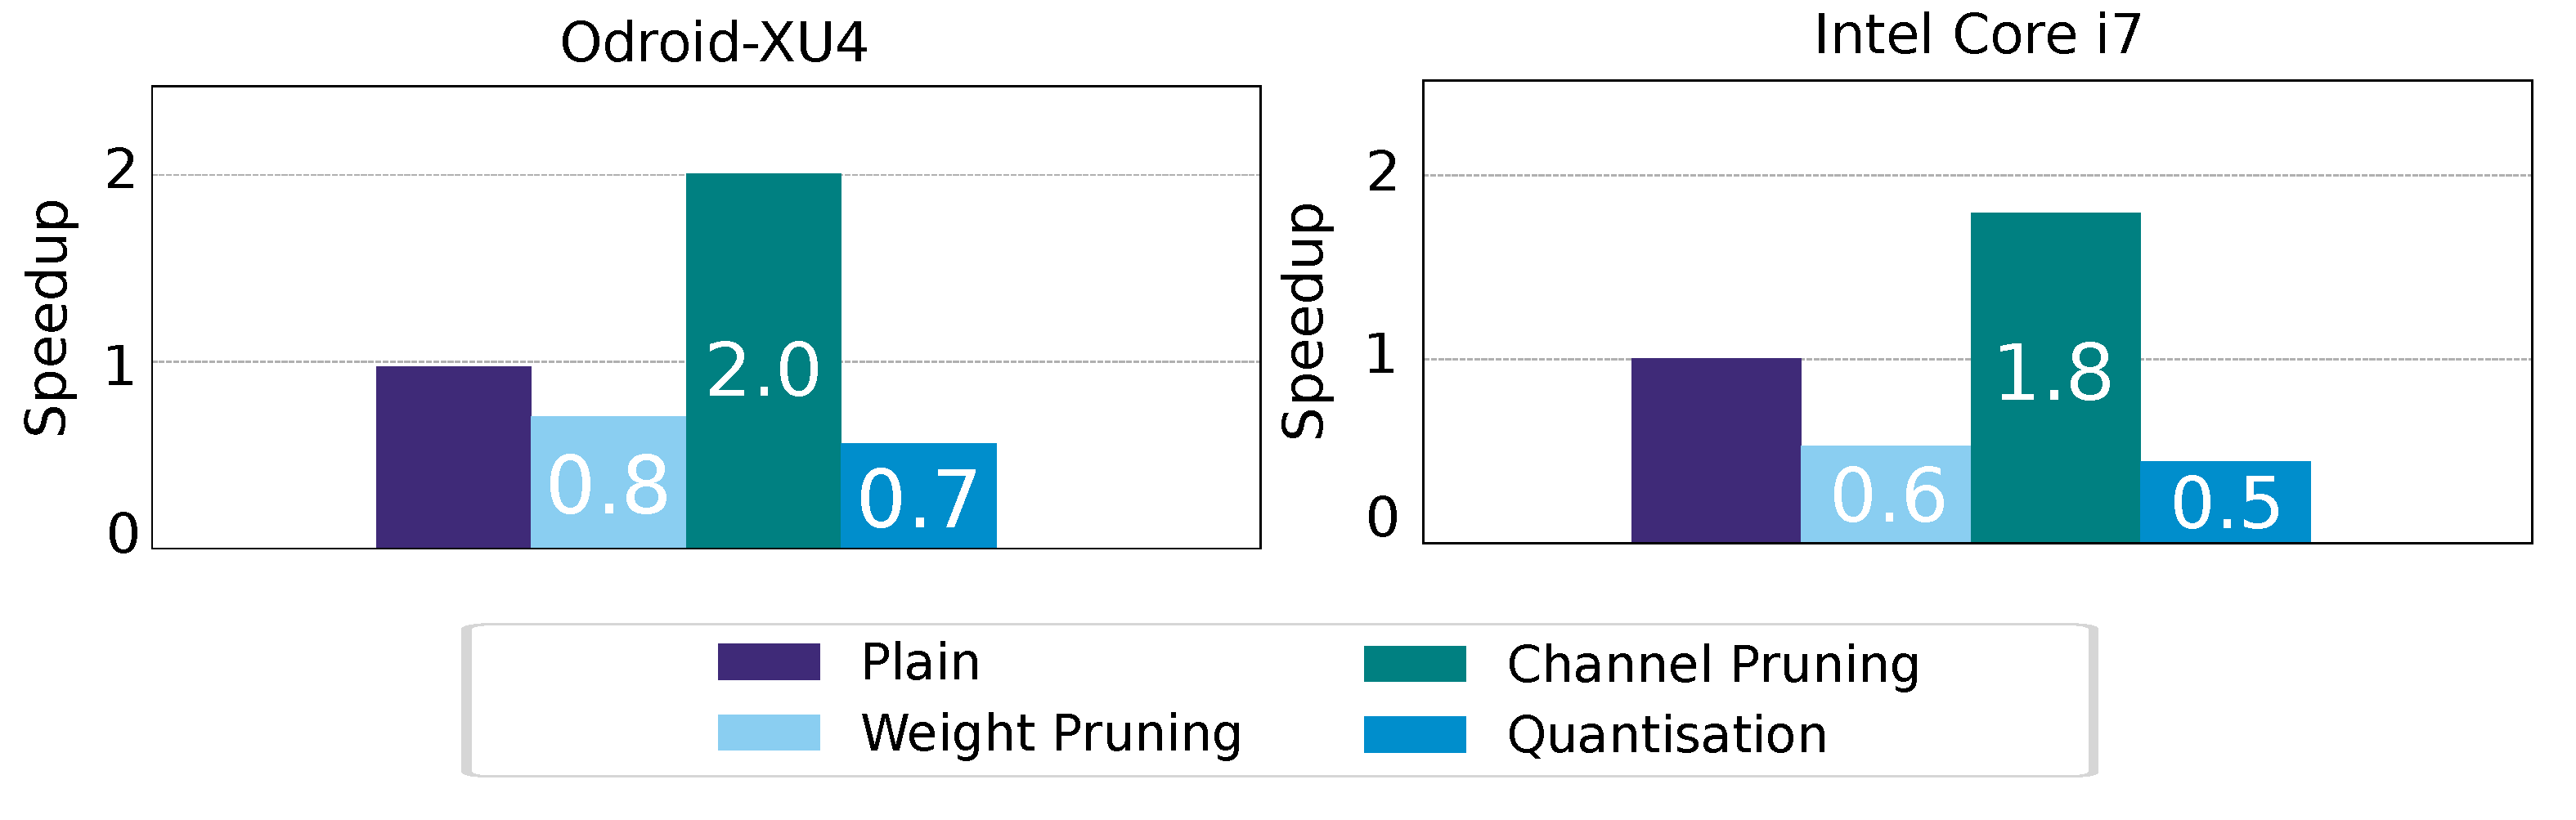
\includegraphics[width=\linewidth]{images/vgg_speedup.pdf}
    \end{figure}
\end{frame}


\begin{frame}{Impact of Compression on Inference Speed}
ResNet-18:
\begin{figure}
    \centering
    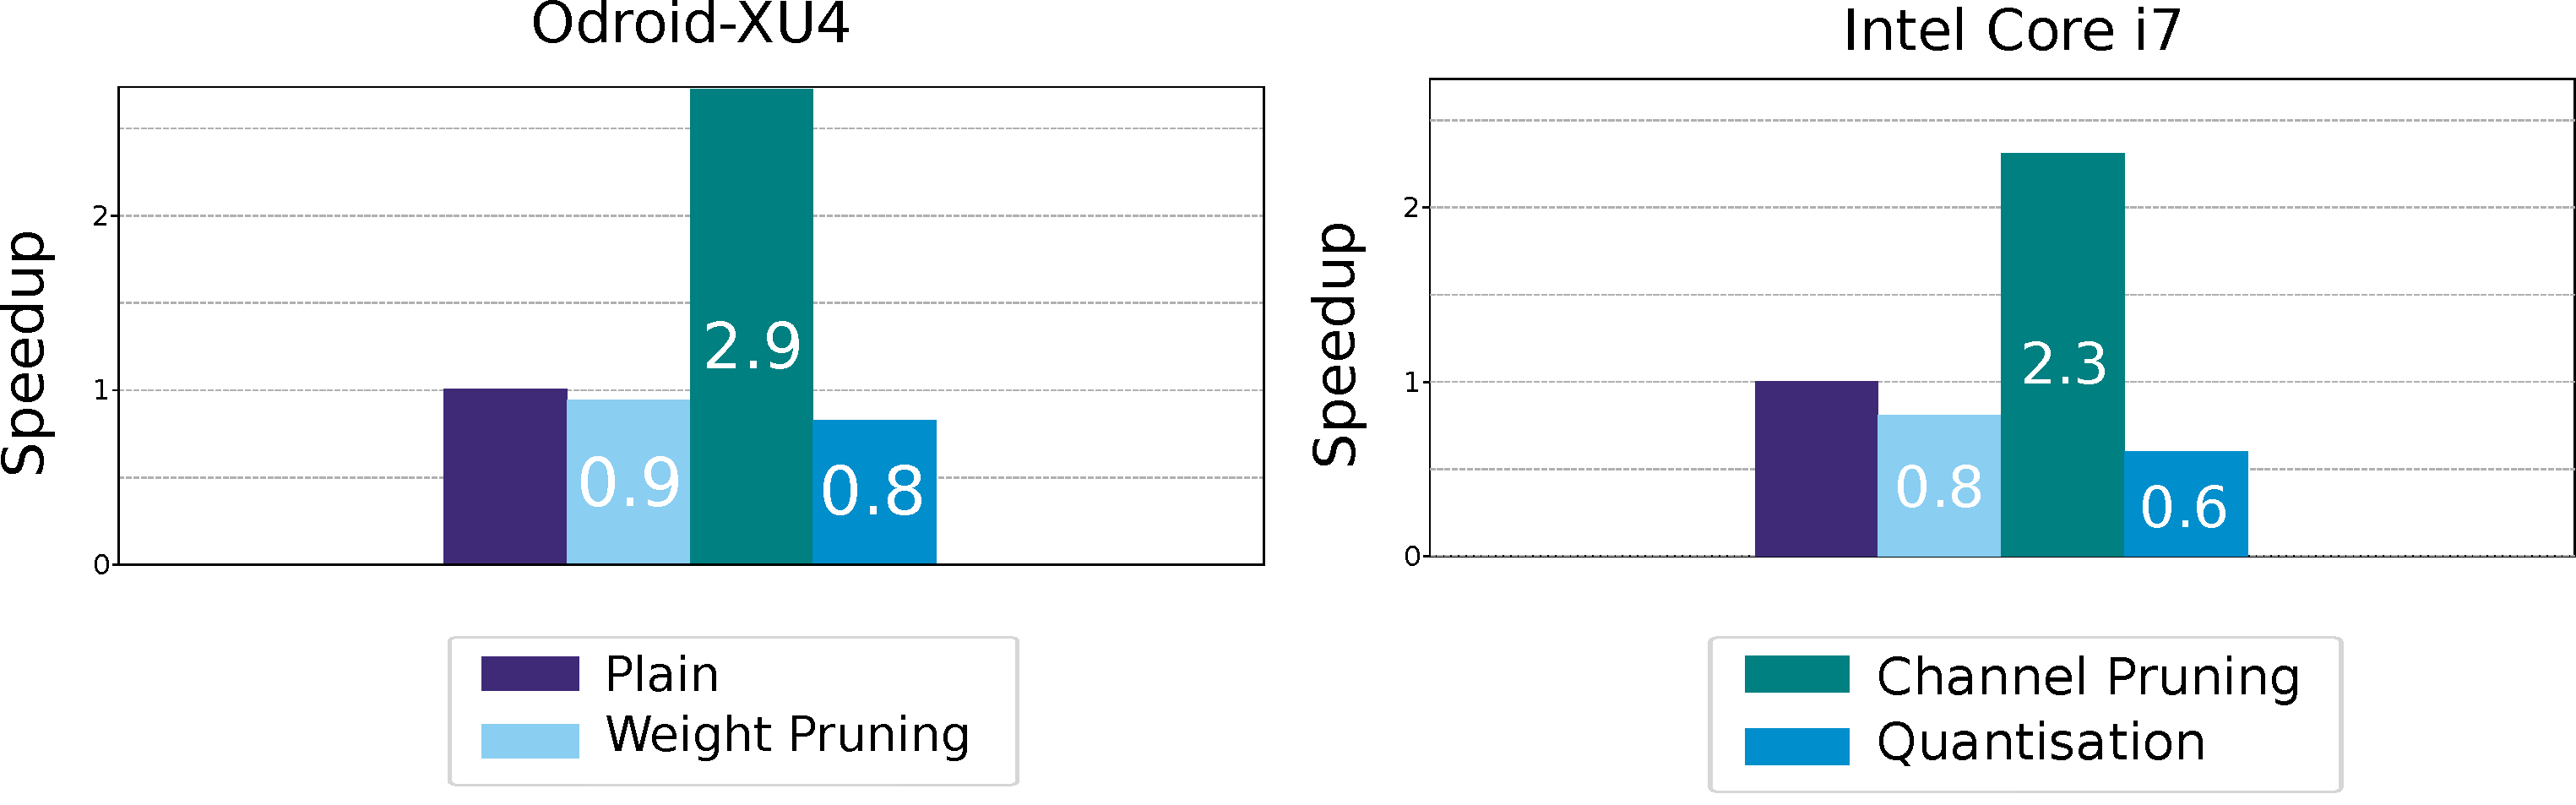
\includegraphics[width=\linewidth]{images/resnet_speedup.pdf}
\end{figure}
\end{frame}


\begin{frame}{Impact of Compression on Inference Speed}
MobileNet:
\begin{figure}
    \centering
    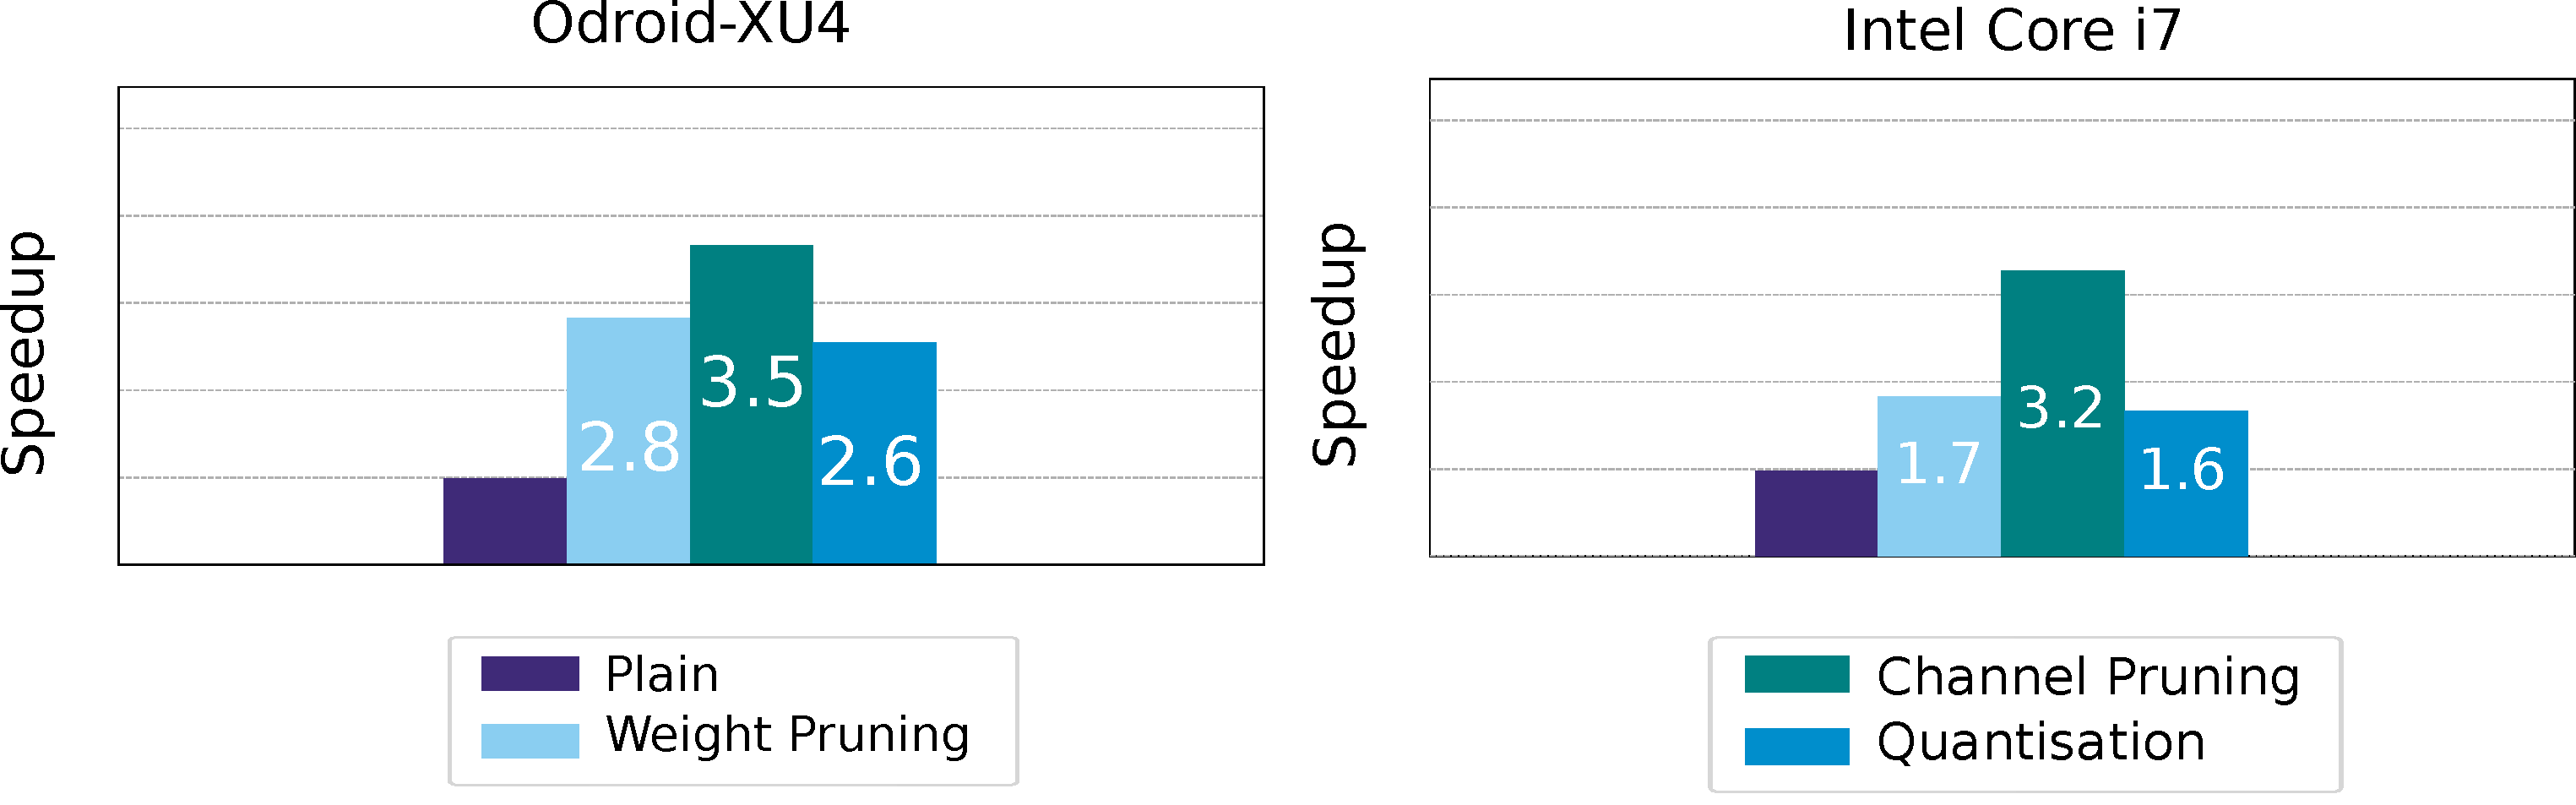
\includegraphics[width=\linewidth]{images/mobilenet_speedup.pdf}
\end{figure}
\end{frame}







\begin{frame}{Experiments}
    
    \begin{figure}
        \centering
        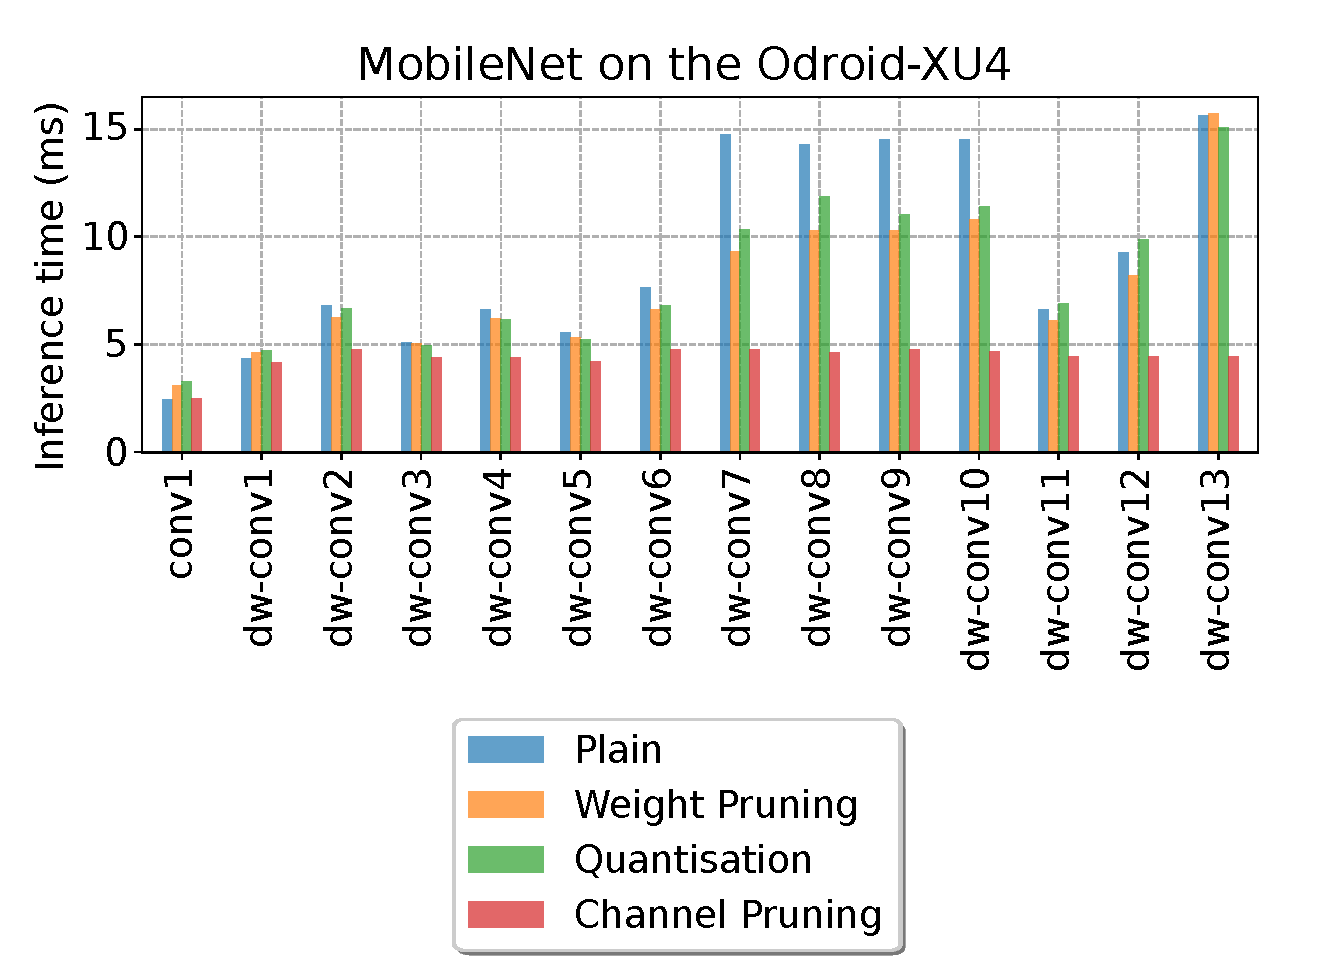
\includegraphics[width=10cm]{images/mobilenet-odroid.pdf}
    \end{figure}
    
\end{frame}


\begin{frame}{Fixing Accuracy}
    
    Now fix the accuracy at 90\% to make results more comparable.
    
    \begin{figure}
        \centering
        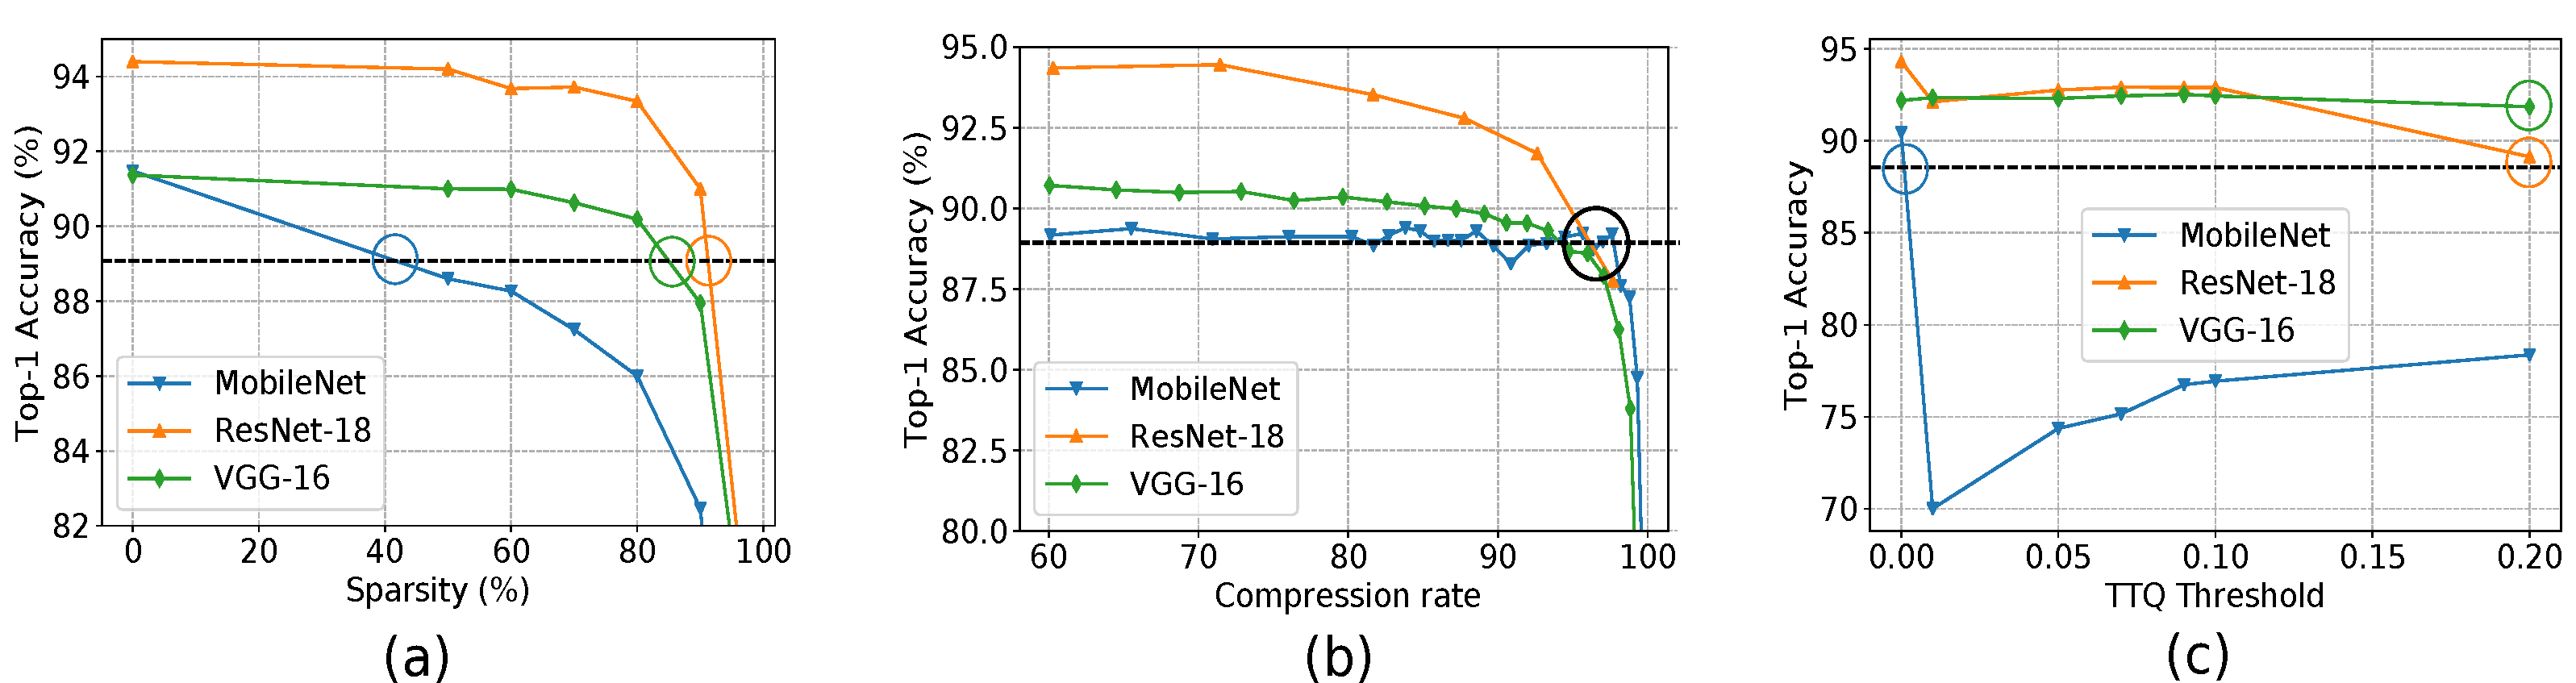
\includegraphics[width=\linewidth]{images/accuracy.pdf}
        \caption{(a) Weight Pruning (b) Channel Pruning (c) Quantisation}
    \end{figure}
    
\end{frame}




\begin{frame}{Comparison at Fixed Accuracy}
    \begin{figure}
        \centering
        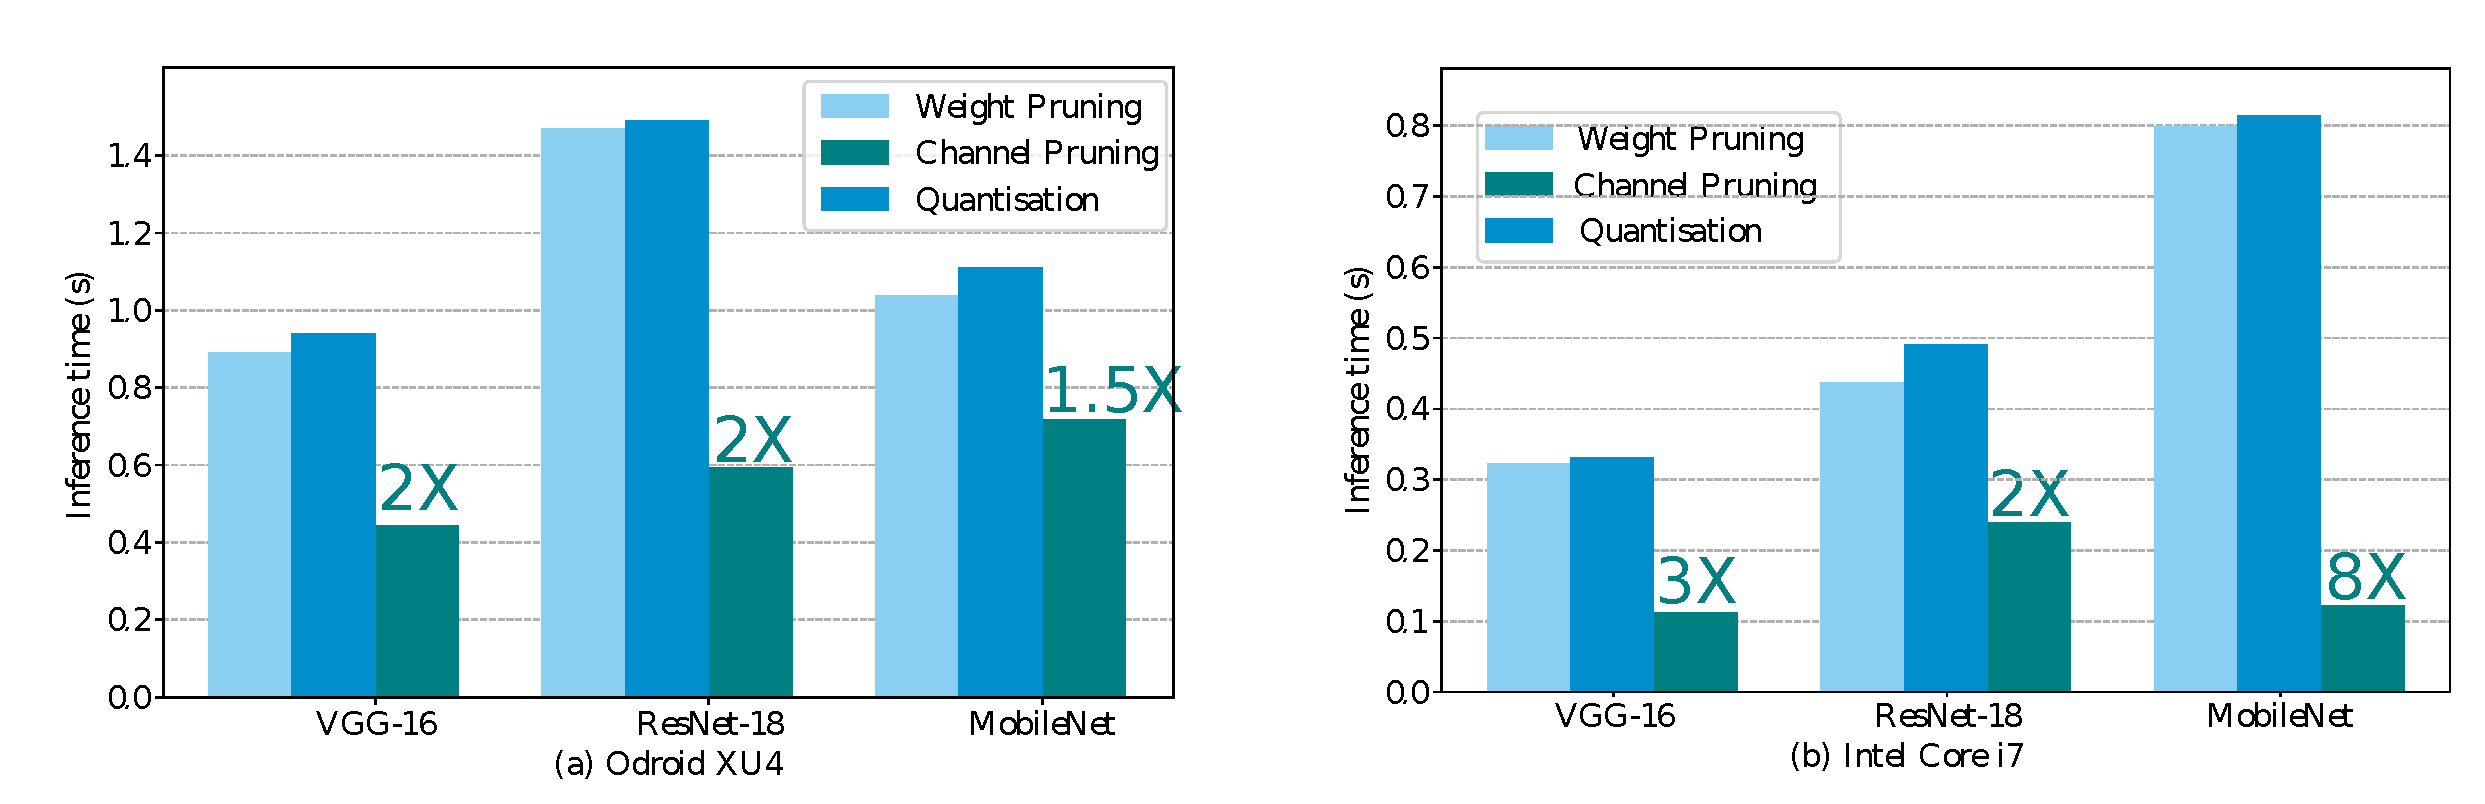
\includegraphics[width=\linewidth]{images/inf-mem2.pdf}
        \label{fig:inf-mem}
    \end{figure}
\end{frame}


\begin{frame}{Acceleration on the Odroid}
    
VGG-16 can run faster than MobileNet on an embedded device for the same accuracy using channel pruning:
    
\begin{center}
    \begin{tabular}{c|c|c|c}
         Model & Accuracy & Size & Speed \\
         \hline
         MobileNet Plain  & 90\% & \textbf{66.3MB}  & 0.6s \\
         VGG-16 C. Pruned & 90\% & 74.9MB  & \textbf{0.4s}\\
    \end{tabular}
\end{center}
  
\end{frame}

\begin{frame}{Parallelisation on ARM Mali GPU}

    \begin{figure}
        \centering
        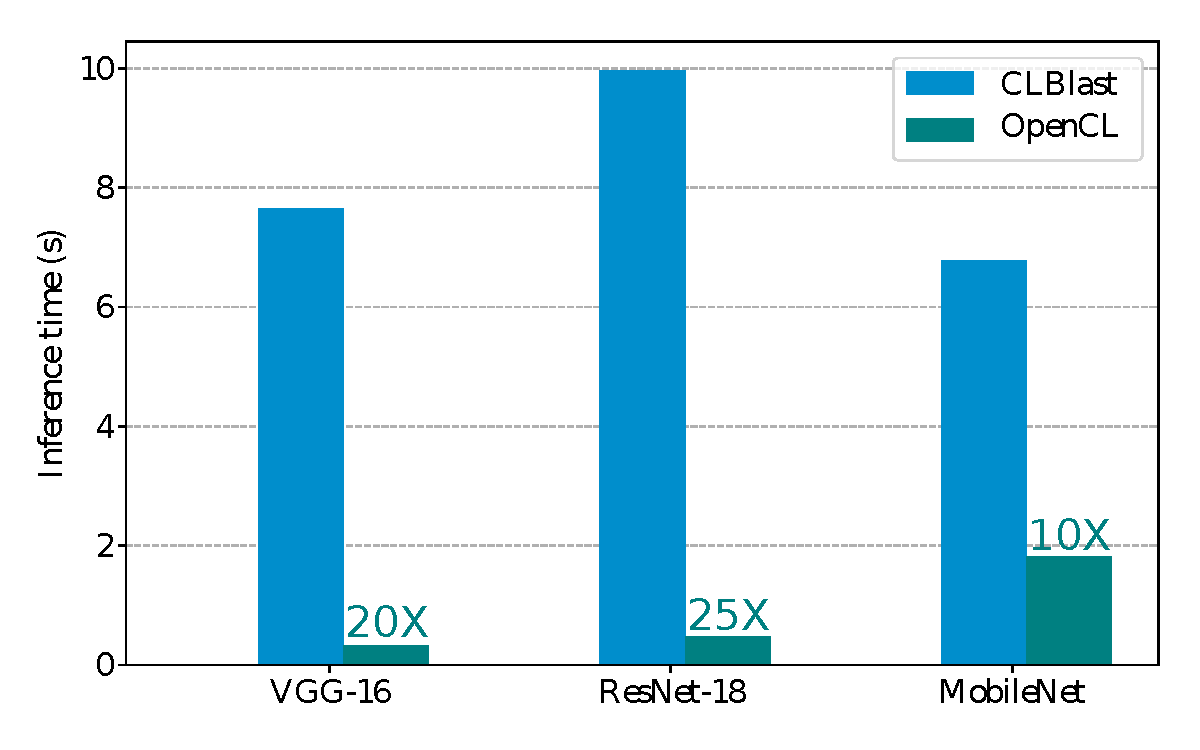
\includegraphics[width=\linewidth]{images/Odroid-GPU.pdf}
        \label{fig:odroid-gpu}
    \end{figure}
    
\end{frame}



\begin{frame}{Conclusion}
    
    \begin{itemize}
        \item Channel pruning is the best, always
        \item FLOPs are \textbf{not} a perfect proxy for inference time
        \item Acceleration patterns are both network \textbf{and} hardware dependent, so you must account for both sides of the stack when deploying deep networks 
    \end{itemize}
    
\end{frame}

\end{document}